\documentclass[
    12pt,                        % Schriftgröße
    ngerman,                     % Neue deutsche Rechtschreibung
    a4paper,                     % Papierformat
    oneside,                     % Einseitig
    titlepage,                   % Eigene Titelseite
    parskip=half,                % Halbe Zeile Abstand zwischen Absätzen
    headings=normal,             % Überschriften nicht zu riesig
    bibliography=totoc,          % Literaturverzeichnis ins Inhaltsverzeichnis
    listof=totoc,                % Abbildungs-/Tabellenverzeichnis ins Inhaltsverzeichnis
    numbers=noenddot,            % Kein Punkt am Ende der Kapitelnummer
    captions=tableabove          % Korrigiert den Abstand über Tabellen
]{scrreprt}

% --- System & Sprache ---
\usepackage[utf8]{inputenc}
\usepackage[T1]{fontenc}
\usepackage{babel}
\usepackage{csquotes}

% --- Typografie & Layout ---
\usepackage{newpxtext,newpxmath}
\linespread{1.05}
\usepackage{microtype}
\usepackage[left=3cm,right=2.5cm,top=2.5cm,bottom=2.5cm]{geometry}
\usepackage{setspace}
\setstretch{1.15}
\usepackage[default]{sourcesanspro}
\usepackage{siunitx}

% --- Grafiken & Tabellen ---
\usepackage{graphicx}
\usepackage{subcaption}
\usepackage{float}
\usepackage{scrhack}
\usepackage{booktabs}
\usepackage{tabularx}
\usepackage{placeins}
\usepackage{etoolbox}

\usepackage{tikz}
\usetikzlibrary{
    shapes.geometric, % Für die Rauten (Entscheidungen)
    arrows.meta,      % Für moderne Pfeilspitzen
    positioning,      % Für relative Platzierung (besser als absolute Koordinaten)
    calc,             % Für Berechnungen von Abständen
    chains            % Optional, falls Sie den Flow automatisch verketten wollen
}

\pretocmd{\section}{\FloatBarrier}{}{}
\pretocmd{\subsection}{\FloatBarrier}{}{}

% --- Externe PDFs einbinden ---
\usepackage{pdfpages}

% --- Abkürzungsverzeichnis ---
\usepackage[printonlyused,withpage]{acronym}

% --- Code Listings (C++ & GLSL) ---
\usepackage[outputdir=build]{minted}
\usepackage{xcolor}

% Theme
\usemintedstyle{manni}
\definecolor{pastelBg}{rgb}{0.96, 0.97, 0.98}
\setminted{
    fontsize=\footnotesize,
    fontfamily=tt,
    linenos=true,
    numbersep=8pt,
    breaklines=true,
    samepage=true,
    frame=leftline,
    framerule=1.5pt,
    framesep=3mm
}
\renewcommand{\theFancyVerbLine}{\ttfamily\tiny\color{gray!80}\arabic{FancyVerbLine}}

% --- Literaturverzeichnis (IEEE) ---
\usepackage[
    backend=biber,
    style=ieee,
    maxcitenames=1,
    mincitenames=1,
    doi=true,
    isbn=false
]{biblatex}

\DefineBibliographyStrings{ngerman}{
    presentedat = {präsentiert auf der\addspace},
    andothers   = {et\addabbrvspace al\adddot}
}

\DeclareSourcemap{
    \maps[datatype=bibtex]{
        \map{
            \step[fieldsource=doi,final]
            \step[fieldset=url,null]
            \step[fieldset=urldate,null]
        }
        \map{
            \step[fieldset=pagetotal,null]
        }
    }
}

\AtEveryBibitem{
    \iffieldundef{url}{
        \clearfield{urlyear}
        \clearfield{urlmonth}
        \clearfield{urlday}
    }{}
}

\addbibresource{Verzeichnisse/literatur.bib}

% --- Hyperlinks (Immer zuletzt laden) ---
\usepackage[hidelinks]{hyperref}


% =====================================================================================================================


\begin{document}

    % --- Zone 1: Keine Seitenzahlen ---
    \pagenumbering{gobble}

    % Erste Seite (Deckblatt)
    
\includepdf[pages={1}]{Verzeichnisse/Bachelor_Deckblatt_Abschlussarbeit.pdf}

    % Zweite Seite (Eidesstattliche Erklärung)
    
\includepdf[pages={2}]{Verzeichnisse/Bachelor_Deckblatt_Abschlussarbeit.pdf}

    \clearpage

    % --- Zone 2: Große römische Zahlen (I, II, III...) ---
    \pagenumbering{Roman}


    \chapter*{Kurzfassung}
    \addcontentsline{toc}{chapter}{Kurzfassung}
    Abstract Placeholder

    \clearpage

    % --- Verzeichnisse ---
    \tableofcontents
    \clearpage
    \listoffigures
    \clearpage
    \listoftables
    \clearpage
    \listoflistings
    \clearpage
    \chapter*{Abkürzungsverzeichnis}
\addcontentsline{toc}{chapter}{Abkürzungsverzeichnis} % Eintrag ins Inhaltsverzeichnis

\begin{acronym}[V-Buffer]
    \acro{ALU}{Arithmetic Logic Unit}
    \acro{API}{Application Programming Interface}
    \acro{CAD}{Computer-Aided Design}
    \acro{CPU}{Central Processing Unit}
%    \acro{FBO}{Framebuffer Object}
    \acro{G-Buffer}{Geometry Buffer}
    \acro{GLSL}{OpenGL Shading Language}
    \acro{GPU}{Graphics Processing Unit}
    \acro{HDR}{High Dynamic Range}
    \acro{LOD}{Level of Detail}
%    \acro{MRT}{Multiple Render Targets}
    \acro{MSAA}{Multisample Anti-Aliasing}
    \acro{MVP}{Model-View-Projection}
    \acro{NPR}{Non-Photorealistic Rendering}
    \acro{PBR}{Physically Based Rendering}
    \acro{RMW}{Read-Modify-Write}
    \acro{ROP}{Raster Operation Pipeline}
    \acro{RT}{Render Target}
    \acro{TAA}{Temporal Anti-Aliasing}
    \acro{V-Buffer}{Visibility Buffer}
    \acro{VRAM}{Video Random Access Memory}
\end{acronym}
    \clearpage

    % --- Zone 3: Arabische Zahlen (1, 2, 3...) ---
    \pagenumbering{arabic}

    % 3-5 Seiten (Final 4)
    \chapter{Einführung}
\label{ch:01_introduction}


\section{Motivation \& Problemstellung}
\label{sec:01_motivation_and_problem}


\section{Ziel der Arbeit \& Forschungsfragen}
\label{sec:01_goal_and_core_questions}


\section{Aufbau der Arbeit}
\label{sec:01_setup}



    % 6-9 Seiten
    \chapter{Grundlagen}
\label{ch:02_grundlagen}

In diesem Kapitel werden die theoretischen Fundamente der untersuchten Rendering-Pipelines definiert.
Dazu gehört die Abgrenzung der verschiedenen Render-Pfade, die Spezifikation der physischen Hardware-Flaschenhälse sowie die Einordnung der Konzepte im Kontext der Stilisierung.


\section{Rendering-Paradigmen und algorithmische Komplexität}
\label{sec:0201_rendering_paradigms_and_complexity}

Dieser Abschnitt widmet sich der formalen Definition und Gegenüberstellung von klassischen und entkoppelten Render-Pfaden unter Berücksichtigung ihrer inhärenten Skalierbarkeit.

\subsection{Forward Rendering}
\label{subsec:020101_forward_rendering_core}
Beschreibung der klassischen Render-Pipeline mit der direkten Berechnung von Geometrie und Schattierung in einem Durchlauf. Erläuterung des theoretischen Aufwandsverhaltens bei steigender Objekt- und Lichtanzahl.

\subsection{Deferred Rendering}
\label{subsec:020102_deferred_rendering_core}
Erklärung der entkoppelten Pipeline und der Zwischenspeicherung von Geometriedaten in separaten Puffern. Aufzeigen der Effizienzgewinne bei der Schattierung durch den Einsatz geometrischer Hilfskörper.


\section{Hardware-Limitierungen und Performance-Metriken}
\label{sec:0202_hardware_limitations_and_metrics}

Dieser Abschnitt spezifiziert die physischen Ausführungseinheiten moderner Grafikhardware, welche die kritischen Engpässe bei der praktischen Ausführung der Render-Pfade bilden.

\subsection{Fragment-Overdraw und Fillrate}
\label{subsec:020201_fragment_overdraw_and_fillrate}
Thematisierung mehrfach gezeichneter Pixel auf identischen Koordinaten. Betrachtung der resultierenden Last für die Füllrate und softwareseitiger Optimierungen wie dem Z-Prepass.

\subsection{Speicherbandbreite (Memory Bandwidth)}
\label{subsec:020202_memory_bandwidth_limitations}
Analyse der Durchsatzgrenzen beim Zugriff auf den Videospeicher. Erläuterung des Lese- und Schreibaufwands durch breite Pufferstrukturen und additive Mischvorgänge.

\subsection{Register Pressure}
\label{subsec:020203_register_pressure_limitations}
Behandlung der limitierten internen Speichereinheiten pro Rechenkern. Beschreibung der Auswirkungen auf die Thread-Parallelisierung bei der Nutzung großer, kombinierter Shader-Programme.

\subsection{Dynamic Branching und Warp Divergence}
\label{subsec:020204_dynamic_branching_and_warp_divergence}
Erläuterung der synchronen Funktionsweise von Thread-Gruppen auf Hardware-Ebene. Beschreibung der sequenziellen Serialisierung bei ungleichen Verzweigungsbedingungen auf Pixelebene.


\section{Grundlagen der Non-Photorealistic Rendering (NPR) Pipeline}
\label{sec:0203_non_photorealistic_rendering_fundamentals}

Dieser Abschnitt kategorisiert die raumbezogenen Konzepte der NPR-Generierung zur selektiven, isolierten Stilisierung von Szenenobjekten.

\subsection{Object-Space- vs. Screen-Space-Stilisierung}
\label{subsec:020301_object_space_vs_screen_space_stylization}
Abwägung von Stilisierungsverfahren direkt auf der dreidimensionalen Szenengeometrie im Vergleich zu nachgelagerten, globalen Filtern auf dem fertigen zweidimensionalen Bild. Gegenüberstellung von präziser Objekttrennung und Laufzeit-Konstanz.

    % 5-8 Seiten (Final 6)
    \chapter{Stand der Technik und verwandte Arbeiten}
\label{ch:std_introduction}

Dieses Kapitel analysiert den aktuellen Forschungsstand zu Forward- und Deferred-Rendering-Architekturen sowie moderne
Industriepraktiken im Bereich hybrider Architekturen und selektiver Stilisierung.
Durch die Betrachtung bestehender Verfahren im Kontext des Non-Photorealistic Renderings (NPR) werden deren
konzeptionelle und leistungstechnische Limitierungen aufgezeigt.
Die Identifikation dieser Schwachstellen sowie der Mangel an empirischen Vergleichsdaten dienen der Definition der
zugrundeliegenden Forschungslücke, legitimieren die in dieser Arbeit durchgeführte holistische Systemanalyse und
ermöglichen die wissenschaftliche Einordnung des eigens entwickelten Evaluations-Frameworks.


\section{Aktueller Forschungsstand zu Forward- und Deferred-Architekturen}
\label{sec:sdt_academic_state}

% Einleitung
Deferred-Rendering-Paradigmen stellen sowohl in der akademischen Forschung als auch in der industriellen Praxis
etablierte Standards dar~\parencite[vgl.][S. 2]{mallettDeferredAdaptiveCompute2018}.
Moderne Echtzeit-Rendering-Pipelines werden maßgeblich von komplexen Beleuchtungsanforderungen getrieben, wodurch das
effiziente Handhaben von Deferred-Architekturen in den Fokus rückt.
Gleichzeitig werden im Bereich des Forward-Renderings durch diverse Optimierungsverfahren die klassischen Schwächen
dieses Ansatzes zunehmend
relativiert~\parencite[vgl.]{olssonClusteredDeferredForward2012, haradaForwardBringingDeferred2012}.
Die Wahl des Rendering-Ansatzes ist in der Praxis stark kontextabhängig und auf die spezifischen Leistungs- und
Qualitätsanforderungen des Zielbildes ausgerichtet.
Folglich existieren sowohl Deferred- als auch Forward-Implementierungen in modernen Engines selten in ihrer reinen
Form~\parencite[vgl.][S. 56]{burnsVisibilityBufferCacheFriendly2013}.
Der wissenschaftliche Diskurs fokussiert sich daher primär auf hybride Lösungsansätze und gezielte Reduktionen
architektonischer Engpässe.

% Forward Rendering
Der primäre architektonische Nachteil naiver Forward-Rendering-Ansätze liegt in der exponentiellen Leistungsdegradation
bei hoher Geometrie- und Beleuchtungskomplexität.
Die algorithmische Komplexität skaliert mit $\mathcal{O}(G \cdot L)$, wobei $G$ die Anzahl der Primitiven und $L$ die
Anzahl der Lichtquellen darstellt~\parencite[vgl.][S. 1]{Thaler2011DeferredRendering}.
Zu dieser Auswertungskomplexität addiert sich eine kombinatorische Explosion der Shader-Permutationen, sobald diverse
Materialeigenschaften und Lichttypen in der Szene verrechnet werden müssen.
Dieser Limitierung liegt die inhärente Eigenschaft von Forward-Pipelines zugrunde, bei hoher Szenen-Entropie
zwangsweise eine gewisse Menge Fragment-Overdraw zu erzeugen~\parencite[vgl.][S. 1]{fatahalianReducingShadingGPUs2010}.
Ansätze wie ein Z-Prepass zur frühzeitigen Verwerfung verdeckter Fragmente gehören in Forward-Pipelines zwar zum
Standard~\parencite[vgl.][S. 57]{burnsVisibilityBufferCacheFriendly2013}, reichen bei hoher Objekt- und Lichtdichte
jedoch nicht aus, um die Effizienz von Deferred-Verfahren zu
erreichen~\parencite[vgl.][S. 4]{Thaler2011DeferredRendering}.
Modernere Paradigmen wie \enquote{Clustered Forward} oder\enquote{Forward+} adressieren dieses Problem, indem
Lichtquellen in 2D-Kacheln oder 3D-Clustern räumlich sortiert
werden~\parencite[vgl.]{olssonClusteredDeferredForward2012, haradaForwardBringingDeferred2012}.
Dies ermöglicht eine Effizienz, die Deferred-Ansätzen nahekommt, während der primäre Vorteil der Forward-Architektur,
die hohe Flexibilität bei der Materialauswertung, erhalten bleibt.

% Deferred Rendering
Deferred-Rendering-Pipelines haben sich in Umgebungen mit hoher geometrischer Komplexität und anspruchsvollen
Beleuchtungsszenarien weitestgehend durchgesetzt, weisen jedoch ebenfalls diverse architektonische Limitierungen
auf.
Der signifikanteste Flaschenhals ist die hohe Auslastung der Speicherbandbreite (Memory Bandwidth), welche durch den
permanenten Schreib- und Lesezugriff auf den G-Buffer induziert
wird~\parencite[vgl.][S. 55]{burnsVisibilityBufferCacheFriendly2013}.
Ein moderner Lösungsansatz ist die Implementierung entkoppelter Architekturen wie des \textit{Visibility-Buffers}
(V-Buffer)~\parencite{burnsVisibilityBufferCacheFriendly2013}, welcher als Shading-Grundlage für
hochkomplexe Geometrie-Pipelines wie der \textit{Nanite}-Architektur in der Unreal Engine 5
dient~\parencite[vgl.][Folie \enquote{Visibility Buffer}]{Karis_Nanite_SIGGRAPH_Advances_2021_final}.
Im Gegensatz zum traditionellen G-Buffer speichert der V-Buffer pro Pixel lediglich minimale geometrische Metadaten
(wie Primitive- und Instanz-IDs) sowie den Tiefenwert.
Die speicherintensive Materialauswertung wird vollständig in einen nachgelagerten Pass verschoben.
Neben der Bandbreitenproblematik existieren in klassischen Deferred-Architekturen zwei weitere Nachteile: die fehlende
native Kompatibilität mit hardwarebasiertem Multisample Anti-Aliasing (MSAA) sowie die Einschränkung bei der Darstellung
transluzenter Oberflächen.
Da die Beleuchtung im Screen-Space berechnet wird, sind die für MSAA erforderlichen Geometriedaten zu diesem Zeitpunkt
verworfen.
Stattdessen müssen temporale Post-Processing-Verfahren (wie TAA) eingesetzt
werden~\parencite[vgl.][S. 5]{Thaler2011DeferredRendering, taaantialiasing}.
Die Evaluierung semitransparenter Geometrie ist im reinen Deferred-Pfad nicht trivial lösbar, da ein Standard-G-Buffer
pro Pixel nur eine diskrete Tiefenschicht vorhält.
Dieses Defizit wird in der industriellen Praxis standardmäßig über einen nachgelagerten hybriden Forward-Pass für
transparente Objekte gelöst~\parencite[vgl.][S. 56]{burnsVisibilityBufferCacheFriendly2013}.

% NPR
Hinsichtlich des Non-Photorealistic Renderings (NPR) unterscheidet die aktuelle Literatur primär zwischen Object-Space-
und Screen-Space-Methoden~\parencite[vgl.][S. 148]{magdicsPostprocessingNPREffects2013}.
Object-Space-Ansätze sind in der Regel in Forward-Pipelines verankert und berechnen Stilisierungen direkt auf der
Geometrie, was eine granulare, objektbasierte Anpassung ermöglicht.
Bei hoher Szenenkomplexität weisen diese Verfahren jedoch eine unzureichende Skalierbarkeit auf, was primär auf den
Fragment-Overdraw bei rechenintensiven Abstraktionseffekten zurückzuführen
ist~\parencite[vgl.][S. 1]{fatahalianReducingShadingGPUs2010}.
Die moderne Rendering-Forschung weicht zur Umgehung dieser Performance-Limits oft auf Screen-Space-Methoden
(Post-Processing) aus, was architektonisch stark den Paradigmen des Deferred-Renderings entspricht.
Wie~\textcite[S. 148]{magdicsPostprocessingNPREffects2013} beschreiben, ist diese Screen-Space-Verarbeitung zwar
sehr efficient, löst jedoch den direkten Bezug zum individuellen 3D-Objekt auf, wodurch etwa die selektive Stilisierung
stark erschwert wird.
Um räumlichen Kontext zurückzugewinnen, wird in der Forschung auf hybride Ansätze wie das \enquote{2.5D NPR}
zurückgegriffen~\parencite[vgl.][S. 17]{Thaler2011DeferredRendering}.
Hierbei fungiert der G-Buffer als Datenquelle für geometrische Metadaten, um komplexe Effekte geometriebewusst im
Screen-Space durchzuführen.
Klassische Deferred-Pipelines weisen in diesem Kontext jedoch eine fundamentale Schwäche bezüglich der Materialvielfalt
auf~\parencite[vgl.][S. 1]{haradaForwardBringingDeferred2012}.
Wie~\textcite[Kap. 2.6]{Thaler2011DeferredRendering} beschreibt, ist das Auswerten zahlreicher spezifischer Materialien
oder Stilisierungen in einem vereinheitlichten Screen-Space-Pass nur unter starken Performance-Einbußen durch
\textit{Dynamic Branching} auf der GPU realisierbar.
In der Konsequenz bleiben performante Stilisierungen bei reinem Deferred-Rendering zumeist auf globale
Post-Processing-Filter beschränkt~\parencite[vgl.][S. 148]{magdicsPostprocessingNPREffects2013}.

% Fazit
Zusammenfassend lässt sich festhalten, dass die aktuelle Forschung zwar diverse architektonische Lösungen für hohe
Geometrie- und Beleuchtungskomplexität sowohl in Forward- als auch in Deferred-Architekturen bietet, die spezifische
Schnittmenge mit selektivem Non-Photorealistic Rendering in Deferred-Pipelines jedoch theoretischen Limitierungen
unterliegt.
Um zu evaluieren, ob und wie diese akademischen Hürden in der Praxis umgangen werden, ist im Folgenden ein genauerer
Blick auf die angewandte Industriepraxis moderner Game-Engines erforderlich.


\section{Verfahren zur selektiven Stilisierung in der Industriepraxis}
\label{sec:sdt_industry_state}


\section{Limitierungen bestehender Ansätze und Identifikation der Forschungslücke}
\label{sec:sdt_usp}

    % 15-20 Seiten
    \chapter{Konzeption und Realisierung}
\label{ch:04_konzeption_realisierung}

Im folgenden Kapitel wird der Aufbau und die technische Umsetzung des in C++ und OpenGL
implementierten Test-Frameworks \ac{HyDra} beschrieben.
Es werden die Struktur der Daten, die Implementierungen der untersuchten Rendering-Pipelines, die Implementierungen der
verwendeten \ac{NPR}-Effekte, die individuellen architektonischen Limitationen sowie die Umsetzung der
Leistungsmessungskomponenten erläutert.
Das implementierte Programm fungiert als Untersuchungs- und Messinstrument, das eine Sandbox-Umgebung bereitstellt, in
der das Verhalten der verschiedenen Rendering-Pipelines erprobt werden kann.

Der Aufbau des \ac{HyDra} Frameworks folgt im Wesentlichen den Kernparadigmen der maximalen Vergleichbarkeit und des
Determinismus.
Das Programm wurde so strukturiert, dass die drei Rendering-Pipelines unter identischen Bedingungen getestet werden
können.


\section{Systemarchitektur und Lebenszyklus}
\label{sec:0401_system_architecture_and_lifecycle}

Die Architektur des \ac{HyDra}-Frameworks ist durch die Entkopplung der logischen Szenenverwaltung (\ac{CPU}-Zustand)
vom eigentlichen Rendering (\ac{GPU}-Dispatch) gekennzeichnet.
Es wird garantiert, dass alle drei Rendering-Pipelines exakt denselben deterministischen Zustand als Eingabedaten
erhalten.
Ziel ist es, etwaigen individuellen \ac{CPU}-Overhead möglichst zu eliminieren.
Für die Deferred-Pipelines wird zudem der Semantische G-Buffer aufbereitet, wofür im Rahmen der Szeneverwaltung
zusätzlich die Vergabe von objektspezifischen \textit{Style-IDs} erfolgt.
Ein weiterer Bestandteil dieser vorbereitenden \ac{CPU}-Logik ist das implementierte View-Frustum-Culling.
Es fungiert als Filter, der die sichtbare Geometrie evaluiert, bevor die Grafikkarte involviert wird.

\subsection{Frame-Lebenszyklus}
\label{subsec:040101_frame_lifecycle}

% Init
Wie in Abbildung~\ref{fig:render_loop_swimlane} dargestellt, durchläuft das Framework vor dem Eintritt in die
Haupt-Rendering-Schleife ein initiales Setup.
Diese Phase erfüllt im Wesentlichen zwei architektonische Aufgaben: Zum einen die Speicherallokation (\ac{VRAM}) der
benötigten \ac{FBO}s, des \ac{G-Buffer}s sowie der \ac{VAO}s und \ac{VBO}s.
Zum Anderen das Laden, Kompilieren und Verlinken aller Shader-Programme inklusive des Uniform-Mappings.
Die in dieser einmaligen Initialisierungsphase definierte Basiskonfiguration kann zur Laufzeit partiell rekonfiguriert
werden (etwa durch dynamische Skalierung der Auflösung oder Anpassung der Bitrate der \ac{G-Buffer}-\ac{FBO}s).
Der Kontrollfluss wird erst an die zyklische Ausführung des Main-Loops übergeben, wenn der initiale Aufbau des \ac{VRAM}
und der Render-Pipelines vollständig abgeschlossen ist.

% Sync.
Am Anfang der Haupt-Rendering-Schleife werden die für die spätere Hardware-Performance-Evaluation relevanten Timer
initialisiert.
Gleichzeitig wird eine explizite Limitierung der Frame-Taktung (\texttt{AwaitCapacity()}) erzwungen, um zu verhindern,
dass die \ac{CPU} der asynchronen \ac{GPU}-Abarbeitung zeitlich zu weit vorausläuft.
Ein derartiger Rückstand der Grafikkarte würde die Latenz- und Profiler-Messungen andernfalls systematisch verfälschen.

% Input.
Im direkten Anschluss steuert ein dezidiertes \texttt{InputController}-Modul die Modifikation des Szenenzustands.
Diese Komponente ermöglicht eine manuelle Interaktion zur Laufzeit, um spezifische Performance-Metriken, visuelle
Artefakte oder systemische Limitierungen der einzelnen Pipelines interaktiv untersuchen zu können.

% Culling & Upload.
Vor der eigentlichen Datenübertragung an die \ac{GPU} wird die Geometrie einem \ac{CPU}-seitigen logischen Pass
unterzogen.
Ein \textit{View-Frustum-Culling} dient hierbei als Filter, um Geometrien, die sich außerhalb des
sichtbaren Bereichs der Kamera befinden, von der weiteren Verarbeitung auszuschließen.
Für die verbleibenden, sichtbaren Entitäten erfolgt anschließend der \ac{PCIe}-Speichertransfer
(\texttt{rlUpdateVertexBuffer()}) der Modell-Transformationsmatrizen und Style-IDs.

% Dispatch.
Nachdem die Datenpräparation auf der \ac{CPU} abgeschlossen ist, wird die Ausführung der selektierten Rendering-Pipeline
orchestriert.
In dieser Phase (\textit{Render Dispatch}) werden die notwendigen Zustandsänderungen der \ac{API} vorgenommen und die
instanziierten Draw-Calls an die \ac{GPU} übermittelt.
Die Grafikhardware übernimmt daraufhin, asynchron zum Main-Thread, die Rasterisierung und Ausführung der definierten
Shader-Logik.
Die exakte Implementierung der Rendering-Pipelines wird in den nachfolgenden Kapiteln evaluiert.

% Telemetry Drain.
Den Abschluss eines Frame-Zyklus bildet die Präsentation des finalen Bildes auf dem Bildschirm.
Zusätzlich werden die asynchronen Hardware-Timer der \ac{GPU} ausgelesen (\texttt{QueryOldestResult()}).
Dieser \textit{Drain}-Prozess erfolgt explizit nicht-blockierend, um die fortlaufende Ausführung der \ac{GPU} für
nachfolgende Messungen nicht durch künstliche \ac{CPU}-Stalls zu unterbrechen.
Hierdurch wird gewährleistet, dass der tatsächliche Render-Overhead der Pipelines isoliert quantifizierbar bleibt.

% Ablaufdiagramm: Frame Lebenszyklus
\begin{figure}[htbp]
    \centering
    \resizebox{\textwidth}{!}{%
        \begin{tikzpicture}[
            >=Latex,
            font=\sffamily,
        % Styles für UML-Elemente
            activity/.style={rectangle, draw=black, thick, rounded corners, inner sep=6pt, minimum width=4.8cm,
            align=center, fill=white},
            crosslane/.style={rectangle, draw=black, thick, rounded corners, inner sep=6pt, minimum width=5.0cm,
            align=center, fill=gray!10},
            branchact/.style={rectangle, draw=black, thick, rounded corners, inner sep=6pt, minimum width=3.0cm,
            minimum height=1.2cm, text width=3.0cm, align=center, fill=white},
            hwblock/.style={rectangle, draw=black, thick, rounded corners, inner sep=8pt, minimum width=6.0cm,
            align=center, fill=gray!20},
            end/.style={circle, draw=black, fill=white, minimum size=0.5cm, double=black, double distance=1.5pt},
            edge/.style={->, thick, rounded corners=3pt},
            dataedge/.style={->, thick, dashed, draw=blue!80!black, rounded corners=3pt}
        ]
            % Hintergrund
            \draw[thick, dotted, gray] (-3.5, 3.0) -- (16.0, 3.0);
            \node[anchor=south west, text=gray, font=\sffamily\bfseries] at (-3.5, 3.1) {Engine Initialisierung};

            \draw[thick, dotted, gray] (-3.5, 0.2) -- (16.0, 0.2);
            \node[anchor=south west, text=gray, font=\sffamily\bfseries] at (9.0, 0.3) {CPU-Logik \&
            Haupt-Render-Schleife};

            \draw[thick, dotted, gray] (-3.5, -8.7) -- (16.0, -8.7);
            \node[anchor=south west, text=gray, font=\sffamily\bfseries] at (-3.5, -8.6) {GPU Pipeline Ausführung};

            \draw[thick, dotted, gray] (-3.5, -17.2) -- (16.0, -17.2);
            \node[anchor=south west, text=gray, font=\sffamily\bfseries] at (-3.5, -17.1) {Abschluss \& Telemetrie};

            % Swimlanes und Header
            \draw[thick, loosely dashed, gray] (7.0, 4.5) -- (7.0, -21.0);
            \node[font=\bfseries\large, anchor=south] at (2.5, 3.8) {CPU};
            \node[font=\bfseries\large, anchor=south] at (11.5, 3.8) {GPU};


            % Knoten Definitionen
            % Phase 1
            \node[activity] (init) at (2.5, 1.8) {Engine Setup \\ \texttt{RenderContext::Init()} \\
            {\scriptsize (Shader \& FBO Allokation)}};
            \node[activity] (sync) at (2.5, -1.2) {Zeitmessung \& Limitierung \\ \texttt{AwaitCapacity()} \\
            {\scriptsize (Blockiert bei GPU-Rückstand)}};
            \node[activity] (input) at (2.5, -3.2) {State-Injektion \\ \texttt{InputController}};
            \node[activity] (culling) at (2.5, -5.2) {Logischer Szenen-Pass \\ \texttt{UpdateVisibility()} \\
            {\scriptsize (Frustum-Culling \& Licht)}};
            \node[crosslane] (upload) at (7.0, -7.2) {VBO Speicher-Transfer (PCIe) \\ \texttt{rlUpdateVertexBuffer()} \\
            {\scriptsize (Szene-Objekte inkl. Style-IDs)}};
            \node[activity] (dispatch) at (2.5, -9.7) {Render Dispatch \\ {\scriptsize (GPU-Kommandos absetzen)}};
            \node[diamond, aspect=2.5, draw=black, thick, align=center, fill=white, inner sep=1pt] (routing) at
            (11.5, -10.7) {Render-Pfad?};
            \node[branchact] (fwd) at (8.3, -12.7) {Forward \\ Pipeline};
            \node[branchact] (uber) at (11.5, -12.7) {Deferred-Uber \\ Pipeline};
            \node[branchact] (vol) at (14.7, -12.7) {Deferred-Volume \\ Pipeline};
            \coordinate (merge_point) at (11.5, -14.2);
            \node[hwblock] (gpu_render) at (11.5, -15.7) {\textbf{Asynchrone Ausführung der Grafikpipelines} \\
            {\scriptsize (Rasterisierung, G-Buffer \& Shader)}};
            \node[activity] (present) at (11.5, -18.7) {Ausgabe des fertigen Frames \\ auf dem Bildschirm};
            \node[activity] (drain) at (2.5, -18.7) {Telemetrie Drain \\ \texttt{QueryOldestResult()}};

            % Kontrollfluss
            \draw[edge] (init) -- (sync);
            \draw[edge] (sync) -- (input);
            \draw[edge] (input) -- (culling);
            \draw[edge] (culling.south) |- (upload.west);
            \draw[edge] (upload.south) |- (dispatch.east);
            \draw[edge] (dispatch.south) -- (drain.north);
            \draw[edge] (drain.south) -- ++(0, -0.4) -| (-4.0, -1.2) -- (sync.west) node[pos=0.25, above=2pt,
            font=\scriptsize\bfseries] {Nächster Frame};
            \draw[edge] (routing.west) -| (fwd.north);
            \draw[edge] (routing.south) -- (uber.north);
            \draw[edge] (routing.east) -| (vol.north);
            \draw[thick] (fwd.south) |- (merge_point);
            \draw[thick] (vol.south) |- (merge_point);
            \draw[thick] (uber.south) -- (merge_point);
            \draw[edge] (merge_point) -- (gpu_render.north);
            \draw[edge] (gpu_render.south) -- (present.north);

            % Datenfluss
            \draw[dataedge] (dispatch.east) -| (routing.north) node[pos=0.25, above=2pt, font=\scriptsize]
                {Push Commands};
            \draw[dataedge] (gpu_render.west) -- (7.0, -15.7) -- (7.0, -18.7) -- (drain.east) node[midway, below=2pt,
            font=\scriptsize] {Timer (bereit)};

        \end{tikzpicture}%
    }
    \caption[UML-Aktivitätsdiagramm des Frame-Lebenszyklus]{UML-Aktivitätsdiagramm des Frame-Lebenszyklus innerhalb des
    HyDra-Frameworks.}
    \label{fig:render_loop_swimlane}
\end{figure}

\subsection{Szeneverwaltung}
\label{subsec:040102_scene_management}

% Einleitung.
Die inhaltliche Verwaltung der dargestellten Szene wird im \ac{HyDra}-Framework von einem dedizierten
Szenenmanager-Modul (\texttt{SceneManager}) übernommen.
Dieses verwaltet den deterministischen Aufbau der Geometrie, insbesondere die Punktlicht-Proxies und die beleuchteten
Geometrien.
Die Geometrien werden prozedural mithilfe eines festgelegten Seeds erstellt.
Es wird sichergestellt, dass jeder Programmaufruf oder jede Änderung durch den Input-Controller zu vollständiger
Szeneparität hinsichtlich der Geometrieverteilung unter den gegebenen Parametern Objektanzahl, Punktlichtanzahl,
Lichtintensität und Objektdichte (Radius des Objektclusters) führt.
Die Szeneparität zwischen Aufrufen und bei Laufzeit-Manipulationen ist während der Performancemessungen hinsichtlich der
untersuchten (Stil-)Entropie, beispielsweise bezüglich der Style-ID-Verteilung oder Geometrieüberlappungen, von
besonders großer Wichtigkeit.

% Datenhaltung.
Die Datenhaltung der Szenegeometrien und Punktlicht-Proxies mitsamt ihrer assoziierten Style-IDs und
Transformationsmatrizen erfolgt in Arrays, die mit der Maximalanzahl der erstellbaren Objekte vorallokiert wurden.
Jeder Geometrie wird ein Index zugewiesen, anhand dessen für jedes Objekt drei Arrays für die Style-ID, die räumliche
Position und die bereits vorab berechnete Transformationsmatrix gespeichert werden
(\ac{SoA}-Muster)~\cite[S.~793]{akenine-mollerRealtimeRendering2019}.

% Entropie.
Hervorzuheben ist hier die Logik bezüglich der Stilentropie-Steuerung, die zwischen gestreuten (hohe Entropie) und
geordneten (niedrige Entropie) Verteilungen wechselt.
Die Zuweisung der Stil-ID erfolgt in Listing ~\ref{lst:style_assignment}.

% Entropie Listing.
\begin{listing}[htbp]
    \begin{minted}{cpp}
float styleId;
if (state.useClusteredStyles) {
    float normAngle = std::fmod(angle, 2.0f * PI);
    if (normAngle < 0.0f)
        normAngle += 2.0f * PI;
    // Divide the 2PI circle by the current number of active styles
    const float slice = (2.0f * PI) / numStyles;
    const int clusterIndex =
        std::clamp(static_cast<int>(normAngle / slice), 0, static_cast<int>(numStyles - 1));
    styleId = activeStyles[clusterIndex];
} else {
    // Distribute using the current pool size
    styleId = activeStyles[i % static_cast<int>(numStyles)];
}
    \end{minted}
    \caption{Berechnung der \texttt{styleId}-Verteilung basierend auf dem Cluster-Status.}
    \label{lst:style_assignment}
\end{listing}

% Culling-Mechanismus.
Die Prüfung der Sichtbarkeit erfolgt mittels eines klassischen Schnitttests der Bounding-Spheres gegen die sechs Ebenen
des Kamera-View-Frustums~\cite[S.~688, Abschn. \textit{Frustum Culling}]{gregoryGameEngineArchitecture2018}.
Darüber hinaus wird die Größe (der Radius) der Light-Volume-Proxies für die Deferred-Volume-Pipeline durch die
Lichtintensität beeinflusst~\cite[S.~891]{akenine-mollerRealtimeRendering2019}.
Im Rahmen des View-Frustum-Cullings werden diese ebenfalls berücksichtigt, um die Darstellung von Lichtern, deren
Wirkungsbereich vollständig außerhalb des Sichtfeldes liegt, zu vermeiden und somit keine unnötigen
Beleuchtungsberechnungen für spätere Performance-Evaluationen zu verursachen.

% Forward Unterschied.
Das Resultat des Szeneaufbaus ist abhängig von der gewählten Rendering-Pipeline.
Während die Deferred-Pipelines die sichtbaren Instanzen als zusammenhängende, lineare Arrays für den Upload erhalten,
erzwingt das Forward-Rendering eine Aufspaltung der Daten.
Der SceneManager durchläuft hierfür eine Iteration über die Style-IDs der sichtbaren Objekte und ordnet diese in
pipelinespezifische Queues (z.\ B.\ \texttt{fwdTransformsGooch}, \texttt{fwdTransformsToon}) an.
Dieser Sortiervorgang auf der \ac{CPU} ist eine architektonische Notwendigkeit des Forward-Ansatzes, um
kostenintensive Shader-State-Changes auf der \ac{GPU} zu
bündeln~\cite[S.~795 u. S.~886]{akenine-mollerRealtimeRendering2019}.

\subsection{Datenfluss der Stilisierung und G-Buffer Layout}
\label{subsec:040103_g-buffer_layout}

% Style-Id Datenfluss.
Für jedes Objekt werden Style-IDs definiert, die die verschiedenen verwendeten Shading-Effekte referenzieren.
Die Definition dieser Style-IDs erfolgt über dynamische Vertex-Buffer (\ac{VAO}s und \ac{VBO}).
Schließlich werden die Style-IDs als instanziierte Vertex-Attribute für jede Geometrie in den Vertex-Shader
übertragen.
Die Style-IDs werden nicht pro Vertex, sondern einmal pro Instanz im Vertex-Shader ausgelesen, um sie
effizient an den Fragment-Shader weiterzureichen, der die \ac{G-Buffer}Textur
erstellt~\cite[S.~797-798]{akenine-mollerRealtimeRendering2019}.
In der Forward Pipeline erfolgt die Mitlieferung der Style-IDs pro verarbeiteter Geometrie direkt in den
Shader-Aufrufen (Draw-Calls).

% G-buffer Layout.
Wie in Tabelle~\ref{tab:gbuffer_layout} aufgezeigt wird für das \texttt{\ac{RT}0} (Albedo) ein 8-Bit-Format
(\texttt{R8G8B8A8}) genutzt.
Für den Normalen-Puffer (\texttt{\ac{RT}1}) wird hingegen ein 16-Bit-Format \texttt{R16G16B16A16} verwendet.
Diese erhöhte Präzision ist eine architektonische Notwendigkeit, da geringere Bittiefen bei den nachfolgenden
Screen-Space-Lichtberechnungen unzureichend sind~\cite[Folie~37]{AdvancesRealTimeRendering}.
Die genauen visuellen Auswirkungen (Banding-Artefakte), die diesen Kompromiss zugunsten einer höheren Speicherbandbreite
erzwingen, werden in der Evaluation der Deferred-Volume-Pipeline in Kapitel~\ref{subsec:040203} im Detail dargelegt.

\begin{table}[htbp]
    \centering
    \caption{Spezifikation des G-Buffer-Layouts im \ac{HyDra}-Framework.}
    \label{tab:gbuffer_layout}
    \small
    \renewcommand{\arraystretch}{1.3}
    \begin{tabularx}{\textwidth}{l | l X X X X}
        \hline
        \textbf{Render Target} & \textbf{Format} & \textbf{Kanal R} & \textbf{Kanal G} & \textbf{Kanal B} &
        \textbf{Alpha} \\
        \hline
        \textit{RT0 (Albedo)}  & \texttt{R8G8B8A8}        & \texttt{BaseColor R}    & \texttt{BaseColor G}
        & \texttt{BaseColor B}    & \texttt{BaseColor A}    \\
        \textit{RT1 (Normal)}  & \texttt{R16G16B16A16}    & \texttt{World Normal X} & \texttt{World Normal Y}
        & \texttt{World Normal Z} & \textbf{Style-ID}       \\
        \textit{Depth}         & \texttt{8-Bit Grayscale} & \texttt{Linear Depth}   & \texttt{--}
        & \texttt{--}             & \texttt{--}             \\
        \hline
    \end{tabularx}
\end{table}

% Die Style-ID.
Der semantische Kern der hybriden Stilisierung liegt in der Persistierung der durchgereichten Instanz-Metadaten.
Wie in Tabelle ~\ref{tab:gbuffer_layout} ersichtlich, wird die komprimierte Style-ID in den ungenutzten Alpha-Kanal des
Normalen-\ac{RT} encodiert.
Durch dieses Mapping stehen den nachgelagerten Deferred-Shadern sämtliche benötigten Metadaten pro Fragment zur
Verfügung.
Dadurch kann die \ac{GPU} im Shading-Pass dynamisch und selektiv den korrekten \ac{NPR}-Algorithmus auswählen.


\section{Pipeline-Architekturen und systematische Restriktionen}
\label{sec:0402_pipelines_and_restrictions}

% Einordnung
In Kapitel~\ref{ch:02_grundlagen}, wurden die theoretischen Paradigmen der grundlegenden Rendering-Pipelines
etabliert.
In diesem Abschnitt werden die tatsächlichen architektonischen Restriktionen der implementierten Renderpfade innerhalb
des \ac{HyDra}-Frameworks analysiert.
Der Fokus liegt demnach nicht auf der grundlegenden Funktionsweise, sondern auf den spezifischen Modifikationen zur
Integration selektiver Stilisierungsprozesse und den daraus resultierenden Hardware-Limitationen.
Im Rahmen der vorliegenden Untersuchung erfolgt eine Analyse der absoluten Skalierungsgrenzen (Bottlenecks) und
spezifischen visuellen Artefakte (Drawbacks) der jeweiligen Architekturen, um das theoretische Fundament für die
quantitative Performance-Evaluation in Kapitel~\ref{ch:05_evaluation} zu legen.

\subsection{Forward Rendering Pipeline}
\label{subsec:040201_forward_pipeline}

% Grundlagen der Verarbeitung.
Die Implementierung der Forward-Pipeline innerhalb des \ac{HyDra}-Frameworks folgt grundsätzlich der klassischen
Standardimplementierung, wie in Kapitel~\ref{ForwardExplanation} dargelegt.
Die verwendete Forward-Pipeline stellt zudem den Basisansatz des naiven Forwards dar und wird entsprechen ohne
zusätzliche Optimierungen wie einen Z-Prepass oder sonstige Varianten implementiert.

% Stilisierung.
Wie in Kapitel~\ref{subsec:040102_scene_management} dargelegt, erfolgt die selektive Stilisierung in der
Forward-Pipeline unmittelbar während der Drawcalls der in Batches instanziierten und von der \ac{CPU}
(dem \texttt{SceneManager}) aufbereiteten Geometrie-Arrays.
Demzufolge wird jedem Objekt der entsprechende Fragment-Shader sowie der damit assoziierte \ac{NPR}-Stil direkt
zugewiesen.

Dieser Ansatz weist, vor allem in Hinblick auf die selektive Stilisierung, allerdings diverse Schwachstellen und
Limitationen auf.
Eine wesentliche Schwachstelle ist die grundlegende Begrenzung in Form von grundlegend vorherrschenden
Uniform-Buffer-Limits.
In der für das Framework gewählten Grafik-\ac{API} OpenGL 3.3 erfolgt die Übergabe der Lichtdaten-Arrays standardmäßig über
\ac{UBO}s, um den \ac{CPU}-seitigen Overhead einzelner Uniform-Zuweisungen pro Lichtquelle zu
minimieren~\cite[S.~798]{akenine-mollerRealtimeRendering2019}.
Die maximale physische Speichergröße, die ein einzelner Uniform-Block umfassen darf, wird treiberseitig durch das
hardwareabhängige Limit \texttt{GL\_MAX\_UNIFORM\_BLOCK\_SIZE} definiert.
Während dieser Wert auf moderner Desktop-Hardware variiert, schreibt die OpenGL-3.3-Spezifikation herstellerübergreifend
eine garantierte Mindestgröße von \texttt{16 KiB} vor~\cite[S.~321, Tab.~6.45]{OpenGL33Core2010}.

Wird jede der Punktlichtquellen im Shader durch eine vereinfachte Struktur aus einer Positions- und einer
Farb-/Intensitätskomponente mit einer Gesamtgröße von \texttt{32 Bytes} abgebildet, lässt sich die theoretisch maximale
Lichtanzahl $N_{\text{Licht}}$ innerhalb des garantierten \ac{API}-Mindestlimits über folgende Relation bestimmen:
\begin{equation}
    N_{\text{Licht}} = \frac{\texttt{GL\_MAX\_UNIFORM\_BLOCK\_SIZE}}{\text{Größe pro Lichtquelle}} =
    \frac{16.384\text{ Bytes}}{32\text{ Bytes}} = 512
    \label{eq:ubo-limits}
\end{equation}

Auf Hardware-Ebene existiert diese Restriktion, weil Uniform-Daten in dedizierten, extrem schnellen On-Chip-Registern
(Constant Registers) der \ac{GPU} gehalten werden müssen~\cite[S.~35]{akenine-mollerRealtimeRendering2019}.
Dieses fundamentale \ac{API}-Limit begründet, warum die Single-Pass-Architekturen des Frameworks
(Forward und Deferred-Uber) auf eine Kapazitätsgrenze von maximal 500 Punktlichtern beschränkt sind, um eine vollständige
Plattformkompatibilität ohne Treiber-Abstürze zu gewährleisten.

% Screen Space Limits.
Eine weitere grundlegende Einschränkung der naiven Forward-Pipeline bezüglich selektiver Stilisierung ist, dass sich
traditionelle Screen-Space- oder Post-Processing-Effekte wie ein Kuwahara-Filter oder Sobel-Outlines nicht selektiv bzw.
partiell anwenden lassen.
Für die Generierung dieser Effekte ist präzises Wissen bezüglich der finalen Szene sowie der Umgebungsgeometrie
erforderlich~\cite[Abschn.~5]{magdicsPostprocessingNPREffects2013}.
Im Rahmen des implementierten Forward-Renderings erfolgt die Anwendung der Shader direkt und isoliert auf die einzelnen
Geometrien innerhalb der Draw-Calls, wodurch keine Umgebungsbezogenen Daten (semantische Objektidentität) des finalen
Bildes während des Shadings auf der \ac{GPU} vorhanden sind.
Eine selektive Realisierung solcher Effekte ist in Forward-Pipelines also schlichtweg nicht möglich.
In Bezug auf den im \ac{HyDra}-Framework implementierten Effekt zur Darstellung von Konturen kann in der
Forward-Pipeline, anstelle der in den Deferred-Pipelines verwendeten Sobel-Outlines (Screen-Space-Methode) das bedingt
gleichwertige Inverted-Hull-Verfahren (Object-Space-Methode) zur Kantenzeichnung verwendet werden
(siehe Abbildung~\ref{fig:040201_outline_comparison}).
Diese nur äußerst bedingte visuelle Parität muss also für etwaige vergleichende Evaluationen berücksichtigt werden.

% Abbildung aus Engine.
\begin{figure}[htbp]
    \centering
    % Linkes Bild
    \begin{subfigure}[b]{0.49\textwidth}
        \centering
        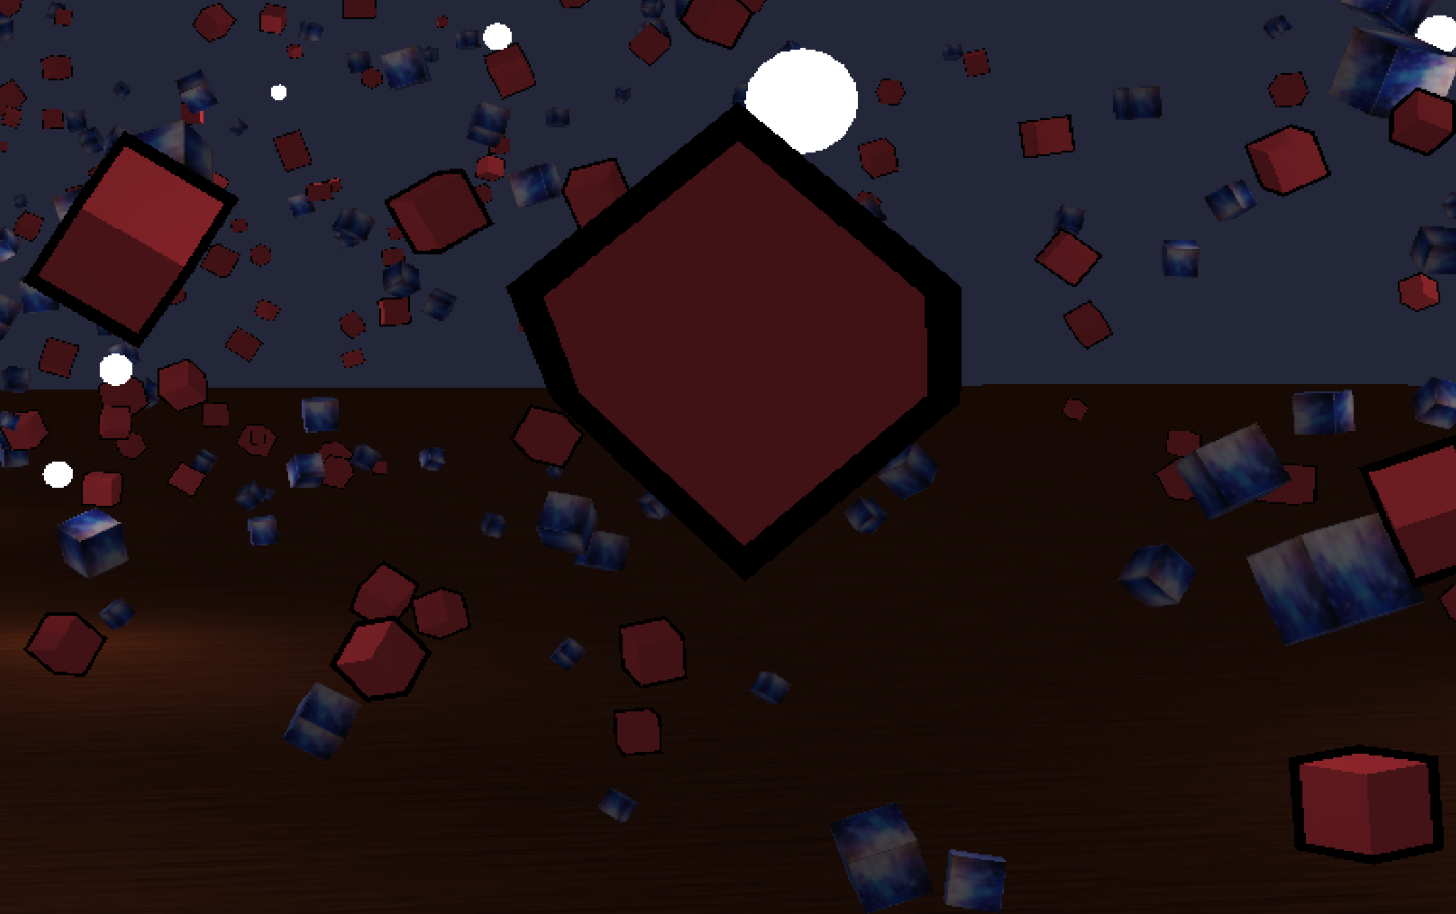
\includegraphics[width=\textwidth]{Abbildungen/IMG-20260711205352333}
        \caption{Inverted-Hull in Forward}
        \label{fig:hydra_inverted-hull}
    \end{subfigure}
    \hfill
    % Rechtes Bild
    \begin{subfigure}[b]{0.49\textwidth}
        \centering
        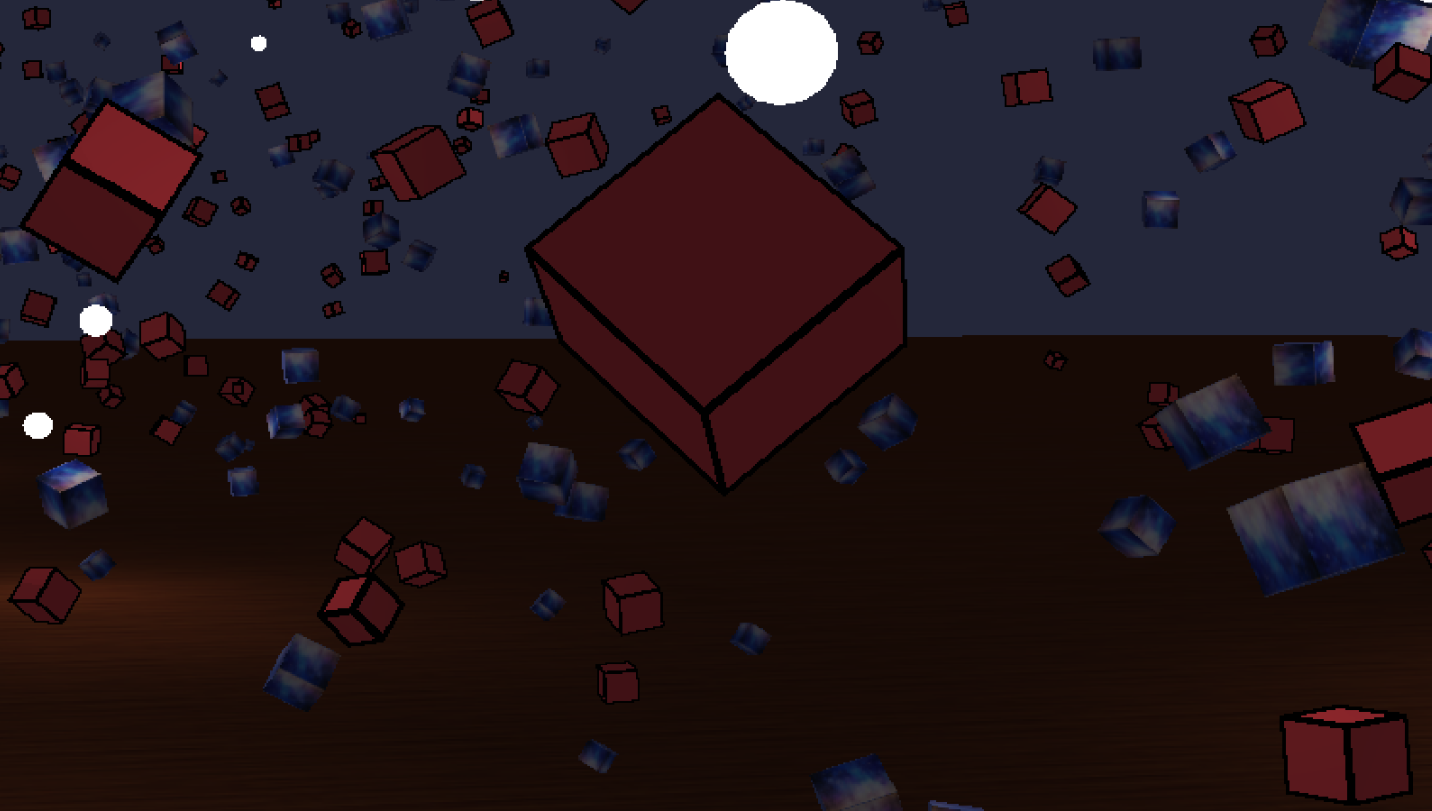
\includegraphics[width=\textwidth]{Abbildungen/IMG-20260711205459842}
        \caption{Sobel-Outlines in Deferred}
        \label{fig:hydra_solebl-outlines}
    \end{subfigure}
    \caption{Vergleich von Kontureffekten in Forward und Deferred mittels Inverted-Hull- und Sobel-Outline-Verfahren.}
    \label{fig:040201_outline_comparison}
\end{figure}




    % 12-15 Seiten (Final 25)
    \chapter{Evaluationen}
\label{ch:05_evaluation}

% Allgemeine Einleitung.
Nach der Definition der softwaretechnischen Realisierung und dem Aufzeigen erster Grenzen und Eigenheiten der
untersuchten Rendering-Paradigmen in Kapitel 4 werden die implementierten Architekturen isolierten Stresstests
unterzogen.
Das primäre Ziel dieses Kapitels liegt in der objektiven Quantifizierung der zuvor theoretisch beschriebenen
Performance-Engpässe unter einer systematischen Skalierung von Szenenkomplexität und Stil-Entropie.
Um die übergeordneten Forschungsfragen belastbar zu beantworten, definiert der erste Abschnitt zunächst die methodischen
Rahmenbedingungen und technischen Spezifikationen des Versuchsaufbaus.
Darauf aufbauend erfolgt die schrittweise Datenauswertung anhand spezifischer Kontrollgruppen und der gezielten
Untersuchung vermuteter Performance-Engpässe, bevor ein abschließender Macro-Benchmark die gewonnenen Erkenntnisse
ganzheitlich evaluiert.


\section{Evaluationsmethodik \& Experimenten-Design}
\label{sec:0501_evaluation_methodology}

% 5.1 Einleitung.
Das in Kapitel 4 konzipierte Test-Framework fungiert im Folgenden als Messwerkzeug für die empirische Analyse der darin
implementierten Rendering-Pipelines.
Für die objektive und isolierte Betrachtung der verschiedenen postulierten Performance-Engpässe definiert der
vorliegende Abschnitt die methodischen Grundlagen.
Dies umfasst die Formulierung der Hypothesen selbst, die exakte Spezifikation des Test-Systems und des
Variablen-Mappings sowie die Orchestrierung des Versuchsablaufs.

\subsection{{Zielsetzung und Hypothesen der Untersuchung}}
\label{subsec:050101_evaluation_tagets_and_hypothesis}

% Evaluationsziel
Wie in Kapitel 3 dargelegt, weisen die theoretischen Architekturparadigmen des naiven Forward-, Deferred-Uber- und
Deferred-Volume-Renderings spezifische Leistungsmerkmale auf.
Das primäre Ziel der nachfolgenden Testreihen besteht in der isolierten Quantifizierung dieser technologischen
Trade-offs.
Es sollen die individuellen Kipppunkte auf Hardware-Ebene lokalisiert und evaluiert werden.
Dadurch soll vermieden werden eine Pipeline den anderen gegenüber, als inhärent überlegen zu präsentieren.

% Technische Hypothesen.
Auf Basis der in Kapitel 3 dargelegten theoretischen Faktenlage werden für die implementierten Rendering-Pipelines
spezifische Leistungshypothesen formuliert.
Diese Annahmen gilt es im Folgenden durch gezielte Evaluationen objektiv zu verifizieren oder zu falsifizieren.
Die empirische Untersuchung beleuchtet dabei gleichzeitig die hardwaretechnischen Grenzen und strukturellen Schwächen
des verwendeten Evaluations-Frameworks \textit{HyDra}.

% Hypothese Forward.
Für die als Referenz gewählte, naive Forward-Rendering-Pipeline werden zwei primäre Leistungsengpässe postuliert.
Auf GPU-Ebene wird bei steigender Szenen- und Beleuchtungskomplexität erwartet, dass die Kombination aus geometrischem
Fragment-Overdraw und der multiplikativen algorithmischen Komplexität der direkten Beleuchtungsberechnung von
$O(\text{Fragmente} \cdot \text{Lichter})$ zu signifikanten Leistungseinbußen führt (\textbf{Hypothese H1.1}).
Hinsichtlich der CPU-Auslastung wird angenommen, dass das CPU-seitige Filtern und Zuordnen von Lichtquellen pro Objekt
sowie das hochfrequente Binden objektspezifischer Licht-Uniforms einen signifikanten API-Overhead provoziert, welcher
die CPU-Zuweisungszeit bei anwachsender Instanzenanzahl nicht-linear skalieren lässt (\textbf{Hypothese H1.2}).

% Hypothese Deferred_Uber.
Für die klassische Deferred-Pipeline mit einfachem Beleuchtungs-Pass monolithischem Uber-Shader wird postuliert, dass
der signifikanteste Leistungsengpass bei einer hohen räumlichen Stil-Entropie auftritt (\textbf{Hypothese H2}).
Wie in den vorangegangenen Kapiteln theoretisch hergeleitet, erzwingen feingranular gestreute NPR-Effekte divergente
Code-Zweige.
Dies führt auf GPU-Ebene unweigerlich zu ineffizienter \textit{Warp-Divergence} (siehe
\ref{sec:0302_industry_state}).
Begleitet wird dieses Phänomen von einem anwachsenden Registerdruck (\textit{Register Pressure}) bei erhöhter
Stil-Vielfalt.
Diese kombinierten Hardware-Flaschenhälse zwingen die Architektur zu einer sequenziellen Abarbeitung der Pixel und
lassen eine messbare Degradation der Shading-Performance bei stark vermischten Effekten erwarten.

% Hypothese Deferred_Volumes.
Für die Deferred-Pipeline auf Basis von Light-Volumes postuliert \textbf{Hypothese H3}, dass diese Architektur eine hohe
Resilienz gegenüber räumlicher Stil-Entropie aufweist und die Branching-Problematik des Uber-Shaders umgeht.
Der primäre Leistungsengpass dieser Methode wird stattdessen in der Sättigung der Speicherbandbreite vermutet.
Das additive HDR-Blending bei einer hohen Anzahl überlappender Light-Volumes provoziert überproportional viele
Read-Modify-Write- (RMW) Zyklen im Framebuffer (VRAM).
Der Uber-Shader umgeht diesen spezifische Speicher-Bottleneck konstruktionsbedingt.

% Abgrenzung sonstiger Limits.
Im vorliegenden Kapitel werden die untersuchten Limitierungen ausschließlich auf Performance-Ebene betrachtet.
Spezifische harte Implementierungsgrenzen der Pipelines (wie etwa die Uniform-Buffer-Limitierungen der Forward- und
Deferred-Uber-Architekturen) sowie etwaige künstlerische Qualitätsengpässe fließen nicht in die Messreihen ein.
Diese Aspekte wurden bereits in Kapitel~\ref{sec:0403_pipeline_implementations} verortet und evaluiert.

\subsection{{Systemkonfiguration und Variablen-Mapping}}
\label{subsec:050102_evaluation_configuration_and_variable_mapping}

% Einleitung
Im Folgenden werden die Referenzdaten der Testumgebung und des verwendeten Software-Stacks beschreiben.
Weiterhin werden die für die testreihen angewendeten unabhängigen Variablen, abhängigen Variablen (Metriken) sowie die
entsprechenden Kontrollvariablen dargelegt udn definiert.

% Einleitung zur Systemkonfiguration.
Die in Tabelle~\ref{tab:hardware_specs} aufgezeigten Hardware-Spezifikationen bestimmen die absoluten physikalischen
Leistungsgrenzen des Systems.
Die in Tabelle~\ref{tab:software_specs} dokumentierten Software-Schnittstellen und Treiber-Versionen definieren die
CPU-seitige Code-Optimierung sowie den grundlegenden API-Overhead.

% Hardware-Tabelle
\begin{table}[h]
    \centering
    \caption{Spezifikation der primären Test-Hardware.}
    \label{tab:hardware_specs}
    \renewcommand{\arraystretch}{1.2}
    \begin{tabularx}{\textwidth}{@{} l X @{}}  % <-- Geändert auf tabularx und \textwidth
        \toprule
        \textbf{Hardware-Komponente}      & \textbf{Spezifikation / Wert}                      \\
        \midrule
        Prozessor (CPU)                   & Intel Core i5-6600K @ 4\times~3.50\,GHz           \\
        Hauptspeicher (RAM)               & 16\,GB DDR4 (Dual-Channel) @ 3000\,MT/s            \\
        Grafikkarte (GPU)                 & NVIDIA GeForce GTX 1660                            \\
        GPU-Architektur                   & Turing (TU116)                                     \\
        VRAM-Kapazität                    & 6\,GB GDDR5                                        \\
        Theoretische VRAM-Bandbreite      & 192,1\,GB/s                                        \\
        Raster Operation Pipelines (ROPs) & 48                                                 \\
        \bottomrule
    \end{tabularx}
\end{table}

% Software-Tabelle
\begin{table}[h]
    \centering
    \caption{Spezifikation der Software-Umgebung und API-Schnittstellen.}
    \label{tab:software_specs}
    \renewcommand{\arraystretch}{1.2}
    \begin{tabularx}{\textwidth}{@{} l X @{}}  % <-- Geändert auf tabularx und \textwidth
        \toprule
        \textbf{Software / API} & \textbf{Version}               \\
        \midrule
        Betriebssystem          & Linux Mint 22.3 (Kernel 6.8.0) \\
        Grafiktreiber           & NVIDIA 595.71.05               \\
        C++ Compiler            & GCC 13.3.0                     \\
        Anwendungs-Framework    & raylib 5.5                     \\
        Grafik-API              & OpenGL 3.3.0 Core Profile      \\
        Shading Language        & GLSL 3.30                      \\
        \bottomrule
    \end{tabularx}
\end{table}

% Einleitung unabhängige Variablen.
Nach der Definition der Hardware- und Software-Spezifikationen erfordert das Evaluation-Design eine exakte Abgrenzung
der unabhängigen Variablen.
Diese Parameter manipuliert das Framework während der Testreihen systematisch.
Es sollen Leistungsgrenzen der Hardware isoliert provoziert werden.
Tabelle~\ref{tab:independent_vars} fasst das Variablen-Mapping zusammen.

% Tabelle der unabhängigen Variablen
\begin{table}[htbp]
    \centering
    \caption{Spezifikation der unabhängigen Variablen und deren Zuordnung zu den Test-Suits.}
    \label{tab:independent_vars}
    \small
    \renewcommand{\arraystretch}{1.1}
    \begin{tabularx}{\textwidth}{@{} l l l >{\raggedright\arraybackslash}X @{}}
        \toprule
        \textbf{Parameter}           & \textbf{Wertebereich} & \textbf{Test-Suite} & \textbf{Beschreibung \& Zweck}                                                                                            \\
        \midrule
        \texttt{activeRenderPath}    & \textit{Enum}         & Alle Suiten         & Die primäre architektonische
        Variable.
        Rotiert durch Forward, Deferred-Uber und Deferred-Volume.\\
        \texttt{currentLodIndex}     & 0 bis 4               & 5.2.1               & Skaliert den geometrischen
        Detailgrad pro Objekt.\\
        \texttt{activeObstacleCount} & bis 50.000            & 5.2.2, 5.2.3, 5.2.3 & Anzahl der gerenderten Instanzen.
        Forciert CPU-Overhead oder Z-Achsen-Overdraw-Dichte.\\
        \texttt{renderResolution}    & 480p bis 4K           & 5.3.1               & Absolute Render-Auflösung zur
        Messung der Fill-Rate. \\
        \texttt{renderFloor}         & \textit{Boolean}      & 5.3.2               & Erzeugt eine Basis-Bandbreitenlast
        (Max Fill-Rate) durch eine raumfüllende Geometrie.\\
        \texttt{activeLightCount}    & 10 bis 5.000          & 5.4.1, 5.4.2.2      & Anzahl der aktiven dynamischen
        Lichter im Frustum.\\
        \texttt{lightIntensity}      & 0,5 bis 20,0          & 5.4.2.1             & Multiplikator für den Lichtradius.
        Forciert RMW-Speicher-Sättigung.\\
        \texttt{useClusteredStyles}  & \textit{Boolean}      & 5.5.1               & Steuert die stilistische Entropie.
        Schaltet zwischen sortierter und gestreuter Verteilung von Effekten um.\\
        \texttt{enableGooch/Toon}    & 1 bis 3 Stile         & 5.5.2               & Stil-Kombinatorik.
        Skaliert die Anzahl der gleichzeitig in einem Frame evaluierten Shading-Modelle.\\
        \texttt{kuwaharaRadius}      & 2 bis 16              & 5.5.3               & Filtergröße für den
        Kuwahara-Kernel.
        Dient der Sättigung der Textur-Bandbreite.\\
        Feature Accumulation         & Pass 1 bis 4          & 5.6               & Kumulative Aktivierung von Geometrie, Basis-Shading und hoher Stil-Entropie über einen determinierten Kamerapfad. \\
        \bottomrule
    \end{tabularx}
\end{table}

% Einleitung abhängigen Variablen
Im direkten Gegenzug zu den manipulierten Parametern erfasst das Telemetrie-Modul des Frameworks eine Reihe
quantitativer Messgrößen.
Diese abhängigen Variablen bilden die empirische Datengrundlage der Evaluationen.
Um die Leistung der Hardware- und Software-Ebenen isoliert beurteilen zu können, werden die Daten pro Frame aggregiert
und zur späteren statistischen Auswertung in das tabellarisch aufgearbeitet.
Tabelle~\ref{tab:dependent_vars} beschreibt die extrahierten Leistungs- und Szenenmetriken.
Die GPU-Laufzeiten werden dabei über asynchrone Hardware-Queries ermittelt, um ein Blockieren der CPU-Pipeline zu
verhindern.

% Tabelle der abhängigen Variablen
\begin{table}[htbp]
    \centering
    \caption{Spezifikation der abhängigen Variablen (Aufzeichnungsmetriken des Telemetrie-Moduls).}
    \label{tab:dependent_vars}
    \small
    \renewcommand{\arraystretch}{1.2}
    \begin{tabularx}{\textwidth}{@{} l l >{\raggedright\arraybackslash}X @{}}
        \toprule
        \textbf{Metrik}           & \textbf{Kategorie} & \textbf{Beschreibung}                                                                                   \\
        \midrule
        \texttt{cpuLogicMs}       & CPU / Host         & Dauer des Logik-Passes (Frustum Culling, Sichtbarkeitsprüfung
        und Matrix-Berechnungen).\\
        \texttt{cpuRenderMs}      & CPU / Host         & Dauer der API-Befehlsübermittlung an die Grafikkarte (Draw Call
        Submission).\\
        \texttt{geomMs}           & GPU / Device       & Dauer des asynchronen Hardware-Queries für den Geometrie-Pass
        (Füllen des G-Buffers).
        Wird für Forward Pipeline nicht befüllt.\\
        \texttt{lightMs}          & GPU / Device       & Dauer des asynchronen Hardware-Queries für die Beleuchtung und
        den NPR-Effekte.
        Forward schreibt hier die kombinierte Last aus Geometrie und Beleuchtung, da Geometrie nicht isoliert werden
        kann.\\
        \texttt{totalGpuMs}       & GPU / Device       & Gesamte GPU-Ausführungszeit des Frames.                                                                 \\
        \texttt{totalFrameTimeMs} & System             & Absolute Frame-Time (Delta Time), gemessen über System-Timer
        (\texttt{std::chrono}).\\
        \texttt{activeInstances}  & Szene              & Anzahl der tatsächlich sichtbaren und verarbeiteten
        Objekt-Instanzen nach dem Frustum Culling.\\
        \texttt{activeTris}       & Szene              & Berechnete Summe der gerenderten Dreiecke (Sichtbare Instanzen
        $\times$ Dreiecke pro Mesh-LOD).\\
        \texttt{currentOverdraw}  & Szene              & Theoretischer Overdraw-Faktor, basierend auf der Frustum-Tiefe
        und der räumlichen Instanzdichte.\\
        \bottomrule
    \end{tabularx}
\end{table}

% Einleitung Kontrollvariablen
Den Abschluss des Variablen-Mappings bilden die Kontrollvariablen.
Diese Parameter definieren die statische Baseline des Frameworks.
Um reproduzierbare Ausgangslagen für alle Messreihen zu garantieren, sind diese Werte eingefroren, sofern die jeweilige
Test-Suite sie nicht explizit als unabhängige Variable überschreibt.
Tabelle~\ref{tab:controlled_vars} fasst die Standardkonfiguration der zusammen.
Besonders kritisch für die Validität der Messungen ist die definierte Warm-up-Phase in Echtzeit.

% Tabelle der Kontrollvariablen
\begin{table}[htbp]
    \centering
    \caption{Spezifikation der Kontrollvariablen und der statischen System-Baseline.}
    \label{tab:controlled_vars}
    \small
    \renewcommand{\arraystretch}{1.2}
    \begin{tabularx}{\textwidth}{@{} l l >{\raggedright\arraybackslash}X @{}}
        \toprule
        \textbf{Kategorie}      & \textbf{Kontrollvariable}          & \textbf{Standardwert (Baseline)}                        \\
        \midrule
        Rendering \& Pipeline   & \texttt{use16BitHDR}               & \texttt{true}                                           \\
        & \texttt{renderResolution}          & $1920 \times 1080$ (1080p)\\
        & \texttt{renderFloor}               & \texttt{true}\\
        \midrule
        Verteilung \& Geometrie & \texttt{activeObstacleCount}       & 5.000                                                   \\
        & \texttt{objectSphereRadius}        & 200,0\\
        & \texttt{currentLodIndex}           & 1\\
        & \texttt{useClusteredStyles}        & \texttt{false}\\
        \midrule
        Licht-Physik            & \texttt{ambientLightStrength}      & 1,0\\
        & \texttt{lightIntensity}            & 2,0\\
        & \texttt{useLightSingularity}       & \texttt{false}\\
        \midrule
        NPR / Stilisierung      & \texttt{enableGooch/Toon}          & \texttt{false}                                          \\
        & \texttt{enableOutlines/Kuwahara}   & \texttt{false}\\
        & \texttt{kuwaharaRadius}            & 4\\
        & \texttt{kuwaharaIntensity}         & 4,0\\
        \midrule
        Test-Orchestrierung     & \texttt{warmupDuration}            & 10,0~Sekunden\\
        & \texttt{captureDuration}           & 1000 Frames\\
        \bottomrule
    \end{tabularx}
\end{table}

\subsection{{Versuchsablauf}}
\label{subsec:050103_evaluateion_procedure}

% Aufwärmphase.
Vor der aktiven Datenaufzeichnung durchläuft das System eine obligatorische Warm-up-Phase von zehn Sekunden.
Dieser Prozess dient dazu, die Hardware-Caches und Textur-Caches
aufzubauen~\parencite[vgl.][Kap. 18.4, Abschn. \textit{Memory Issues}]{akenine-mollerRealtimeRendering2019}.
Hierdurch werden inkonsistente Frametimes, die durch asynchrone Ladevorgänge, späte Speicherallokationen oder
aufgeschobene Statusänderungen des Grafiktreibers in den ersten Frames
entstehen~\parencite[vgl.][Kap. 18.4.2, Abschn. \textit{State Changes}]{akenine-mollerRealtimeRendering2019},
für die Messung exkludiert.
Beim Wechseln von Rendering-Pipelines oder beim Voranschreiten abhängiger Schritt-Variablen wird ebenfalls eine
Warm-up-Pause von zehn Sekunden erzwungen.


% Sampling.
Nach der Warm-up-Phase startet die Sampling-Phase mit einer festgelegten Dauer von 1000 Frames.
Die Kamera wird eingefroren (Ausnahme: Evaluation 5.6).
Das Telemetrie-Modul fragt nun jede der definierten abhängigen Variablen pro Frame ab und akkumuliert die Rohdaten in
dedizierten Arrays zur späteren Exportierung.

% Datenaufbereitung.
Die final präsentierten Graphen und Messergebnisse basieren auf arithmetischen Mittelwerten der Sampling-Phase.
Zur Identifikation und Bereinigung unvorhersehbarer Micro-Stutterer (\textit{Frame-Rate Spikes}) wird die
Standardabweichung der Frame-Zeiten
berechnet~\parencite[vgl.][Abschn. 8.5.2.2]{gregoryGameEngineArchitecture2018}.
Für jede Parameter-Konfiguration bildet die Menge der erfassten Frame-Metriken den initialen Datensatz $X$.
Aus diesem werden gruppenbasiert der empirische Mittelwert $\mu$ sowie die Standardabweichung $\sigma$ berechnet.
Ein individueller Messwert $x_i \in X$ wird ausschließlich dann in die finale Kurvengenerierung einbezogen, sofern die
folgende Bedingung erfüllt ist:

\begin{equation}
    \mu - 3\sigma \le x_i \le \mu + 3\sigma
\end{equation}

Datenpunkte außerhalb dieses Intervalls klassifiziert der Algorithmus als statistische Ausreißer und verwirft diese für
die finale Auswertung.
Dieser Schritt garantiert, dass die später präsentierten Messdaten das rein architektonische und algorithmische
Skalierungsverhalten der Rendering-Pipelines abbilden.


\section{{Geometrische Dichte und Overdraw}}
\label{sec:0502_geometry_eval}

Im Rahmen des nachfolgenden Kapitels werden Benchmarks und Erkenntnisse präsentiert, die dazu dienen, geometriebedingte
Performance-Bottlenecks innerhalb der untersuchten Rendering-Pipelines zu evaluieren.
Der Fokus liegt primär auf der Isolation der Hardware-Rasterizer und der CPU-Draw-Call-Aufwände.

\subsection{{LOD (Mikro-Geometrie)}}
\label{subsec:050201_lod_eval}

\begin{figure}[htbp]
    \centering
    
\includegraphics[width=0.9\linewidth]{Abbildungen/5-2-1_bottleneck_divergence}
    \caption[Geometrische Skalierung bei variierendem Detailgrad]{Messung der GPU- und CPU-Laufzeiten bei einer
    LOD-Skalierung von 24.000 bis 16,38 Mio. Dreiecken und einer konstanten Objektanzahl von 2.000 zur Isolation des
    Hardware-Rasterizers.}
    \label{fig:5_2_1_bottleneck_divergence}
\end{figure}

\subsection{{Object Count Limit}}
\label{subsec:050202_obejct_count_eval}

\begin{figure}[htbp]
    \centering
    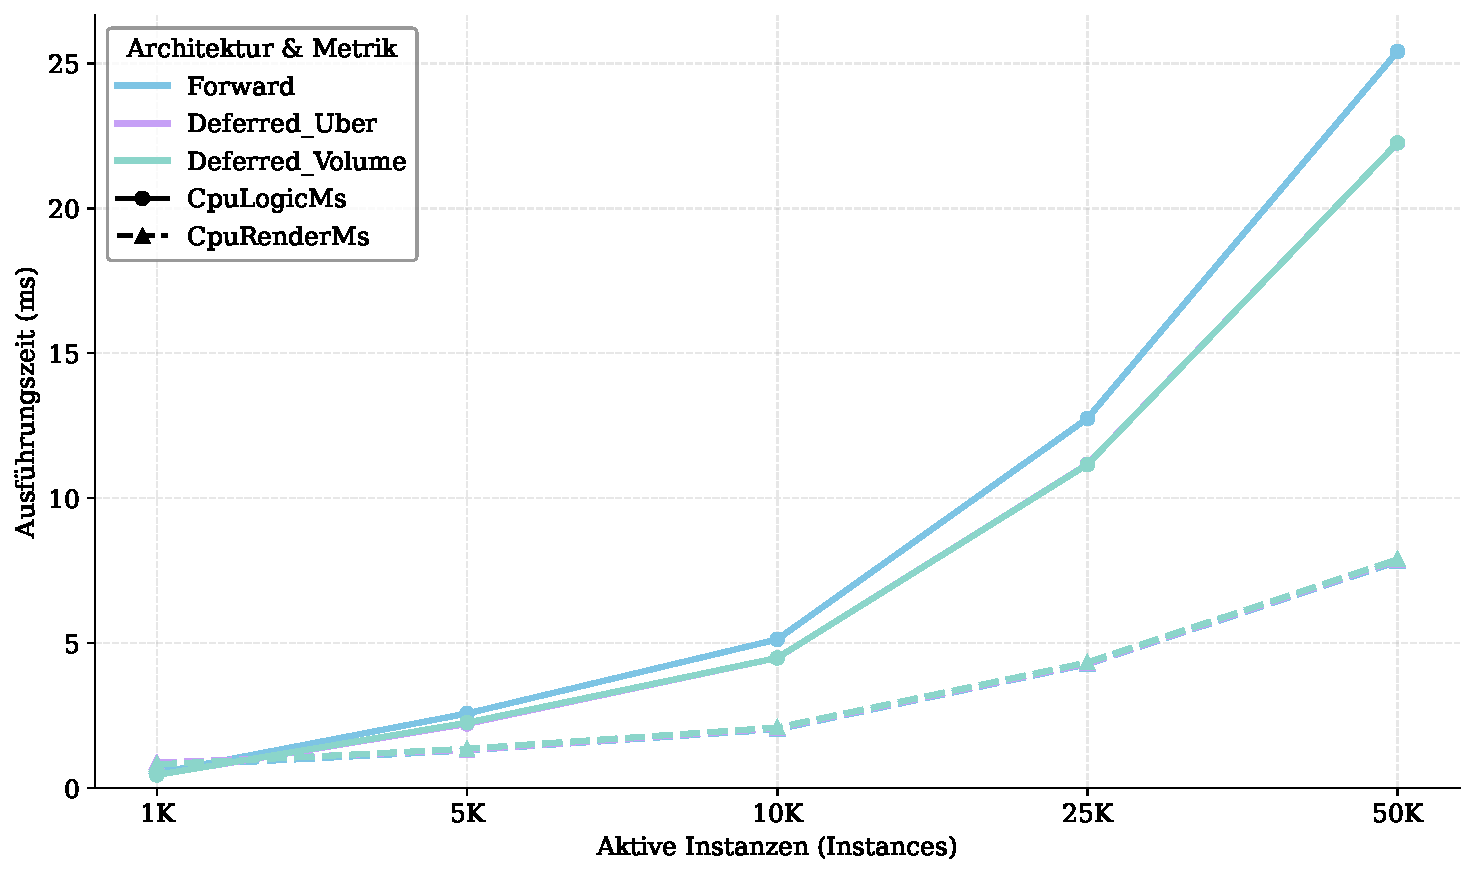
\includegraphics[width=0.9\linewidth]{Abbildungen/5_2_2_cpu_scaling_logic_vs_render}
    \caption[Objektanzahl-Limitierung im CPU-Dispatch]{Messung von \texttt{CpuLogicMs} und \texttt{CpuRenderMs} bei
    einer Skalierung von 1.000 bis 50.000 Instanzen zur Isolation der CPU-Architektur.}
    \label{fig:5_2_2_cpu_scaling_logic_vs_render}
\end{figure}

\subsection{{Overdraw-Dichte}}
\label{subsec:050203_overdraw_eval}

\begin{figure}[htbp]
    \centering
    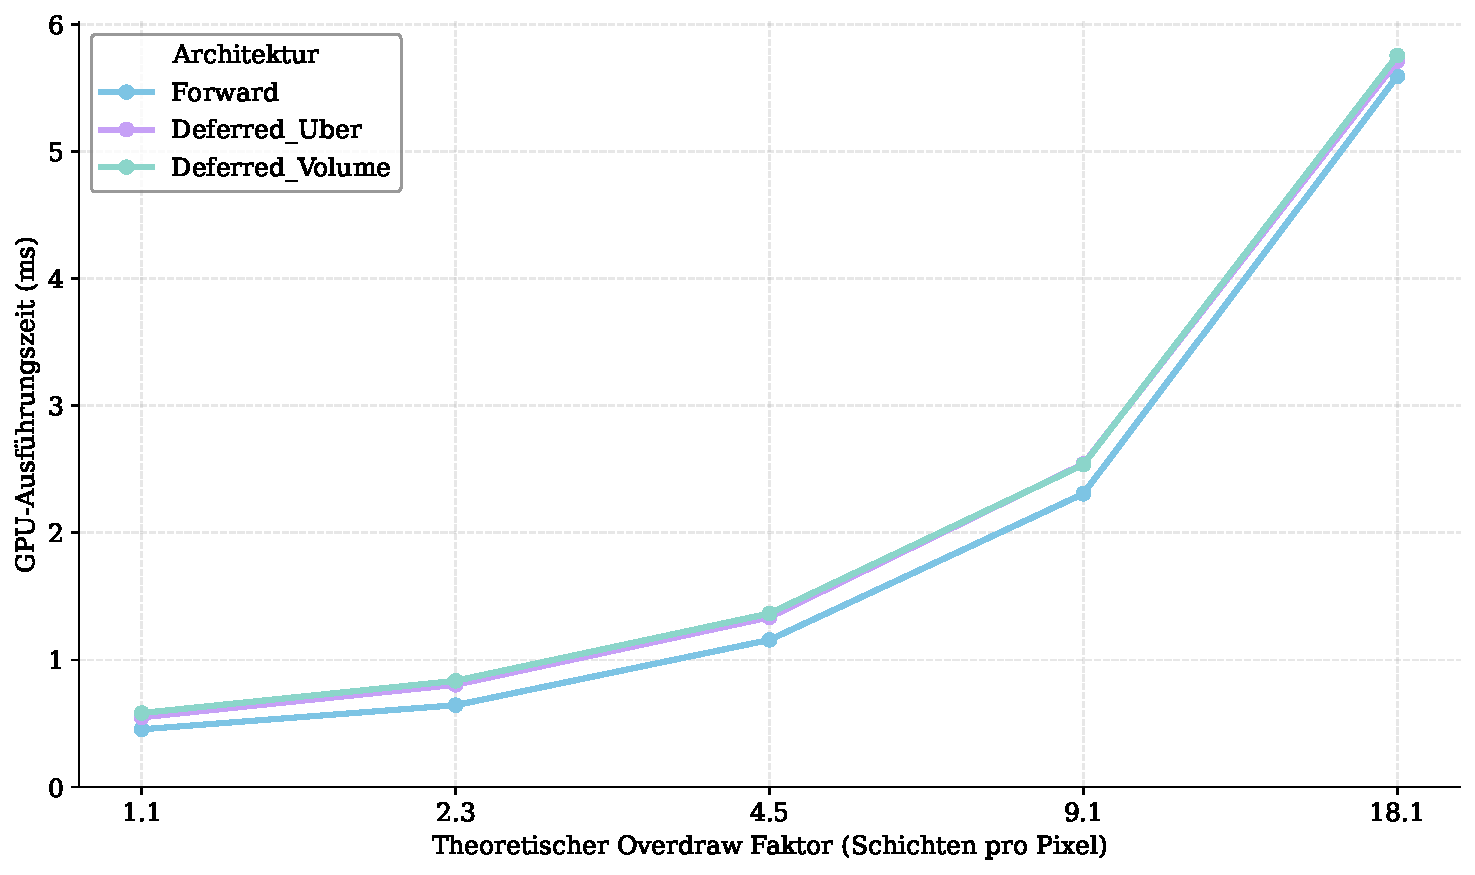
\includegraphics[width=0.9\linewidth]{Abbildungen/5_2_3_overdraw_fillrate_scaling}
    \caption[Overdraw-Skalierung bei steigender Tiefenkomplexität]{Messung der GPU-Ausführungszeit in Abhängigkeit vom
    theoretischen Overdraw-Faktor (1,1 bis 18,1 Schichten pro Pixel) bei einer Skalierung von 2.000 bis 32.000
    Instanzen.}
    \label{fig:5_2_3_overdraw_fillrate_scaling}
\end{figure}


\section{{Bandbreite und Auflösung}}
\label{sec:0503_brandwidth_resolution_eval}

In dem nachfolgenden Kapitel werden Benchmarks und Erkenntnisse präsentiert, die dazu dienen, die
bandbreitenspezifischen Limitierungen auszuloten.
Im Rahmen der Analyse werden die API und die Speicherkosten des G-Buffers sowie der zunehmende ALU-Aufwand des
Forward-Rendering evaluiert.

\subsection{{Auflösung}}
\label{subsec:050301_resolution_eval}

\begin{figure}[htbp]
    \centering
    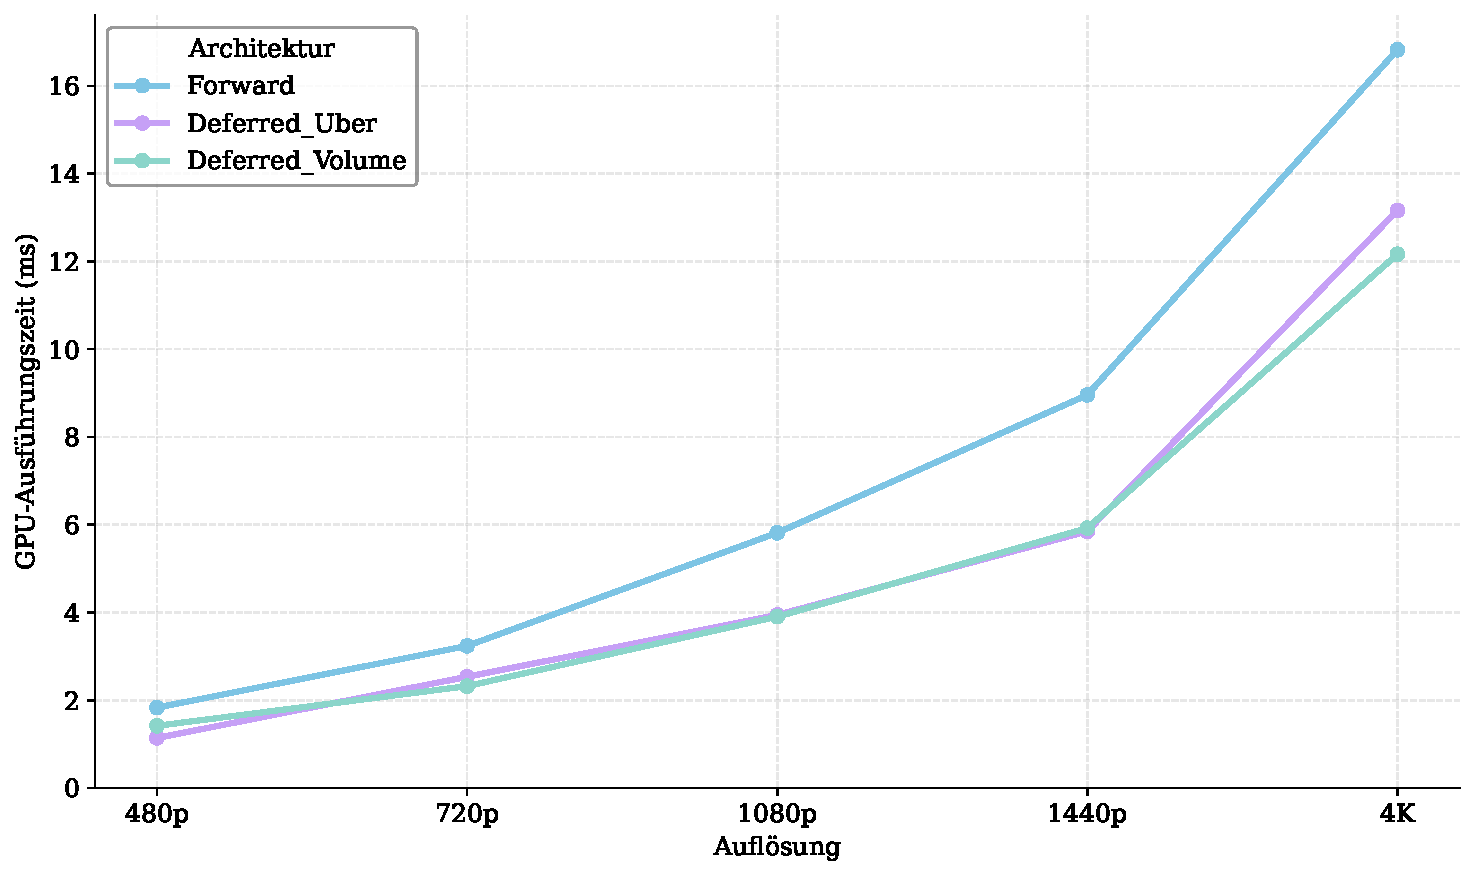
\includegraphics[width=0.9\linewidth]{Abbildungen/5_3_1_resolution_scaling_crossover}
    \caption[Auflösungsskalierung unter konstanter Beleuchtungslast]{Messung der GPU-Ausführungszeit in Abhängigkeit von
    der Framebuffer-Auflösung (480p bis 4K) unter einer statischen Last von 100 Lichtquellen.}
    \label{fig:5_3_1_resolution_scaling_crossover}
\end{figure}

\subsection{{Bandbreiten}}
\label{subsec:050302_bandwidth_eval}

\begin{figure}[htbp]
    \centering
    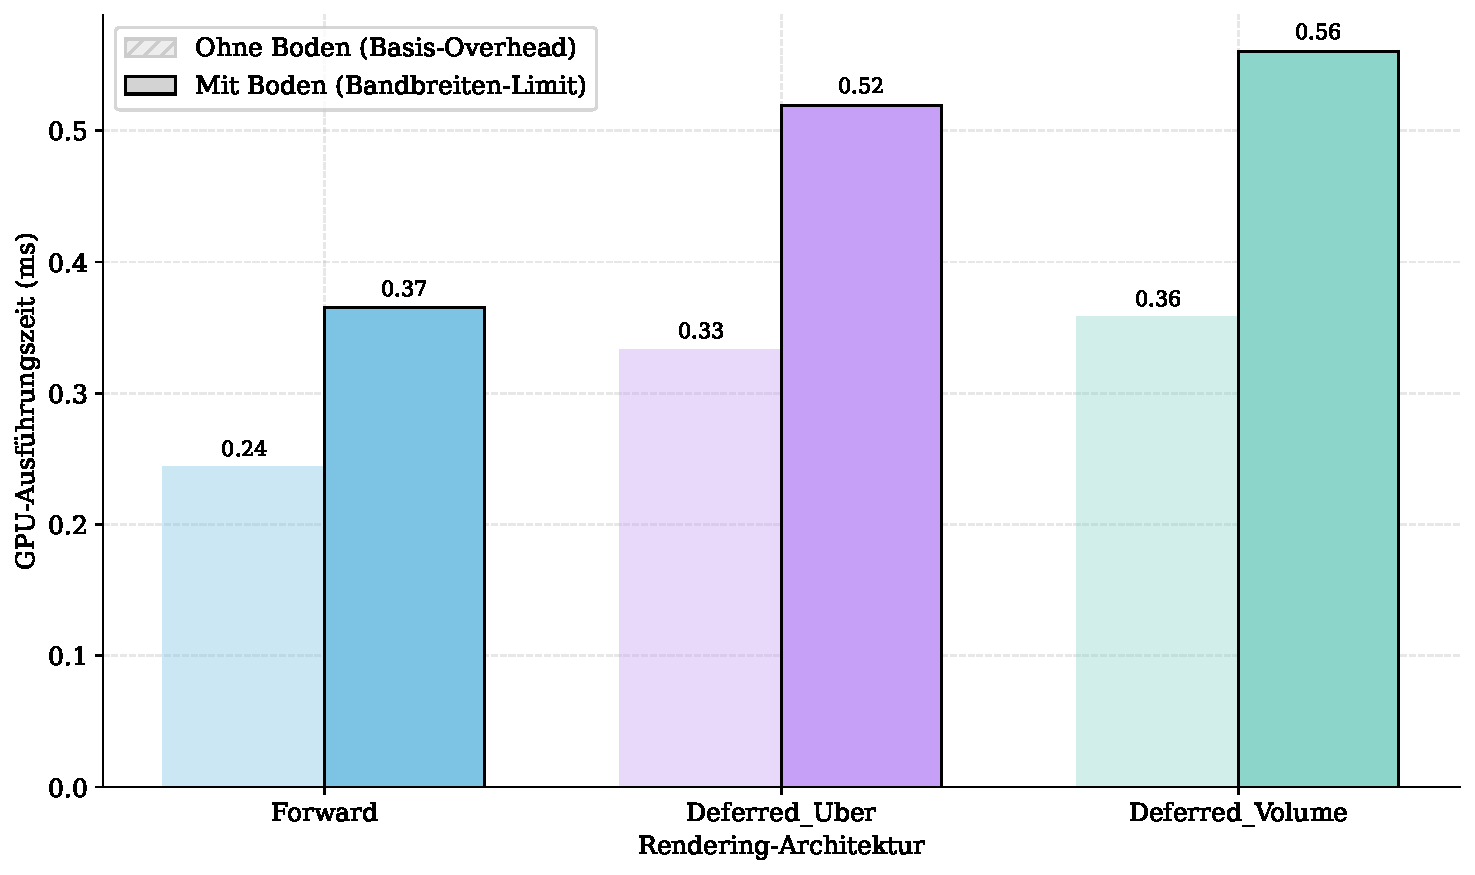
\includegraphics[width=0.9\linewidth]{Abbildungen/5-3-2_BaseBandwidthTax_Means}
    \caption[Basis-Bandbreitenkosten der Rendering-Architekturen]{Vergleich der GPU-Ausführungszeit zwischen minimaler
    Geometrielast (Basis-Overhead) und vollflächiger Screen-Space-Abdeckung (Bandbreiten-Limit) ohne Beleuchtung zur
    Isolierung der G-Buffer-Speicherbandbreite.}
    \label{fig:5_3_2_base_bandwidth_tax_means}
\end{figure}


\section{{Beleuchtung}}
\label{sec:0504_lighting_eval}

Im nachfolgenden Kapitel werden Benchmarks und Erkenntnisse präsentiert, die dazu dienen, die beleuchtungsspezifischen
Limitierungen zu ermitteln.
Da Deferred Rendering im Bereich der Beleuchtungsberechnung signifikante Vorteile verspricht, sollen im Folgenden die
genauen architektonischen Crossover-Points ermittelt werden, ab denen die Deferred-Pipelines die Forward-Pipelines
übertreffen.
Auf Hardware-Ebene werden im Rahmen der vorliegenden Untersuchung die ALU- und ROP-Limits mithilfe der nachfolgenden
Benchmarks evaluiert.

\subsection{{Lichtanzahl}}
\label{subsec:050401_light count_eval}

\begin{figure}[htbp]
    \centering
    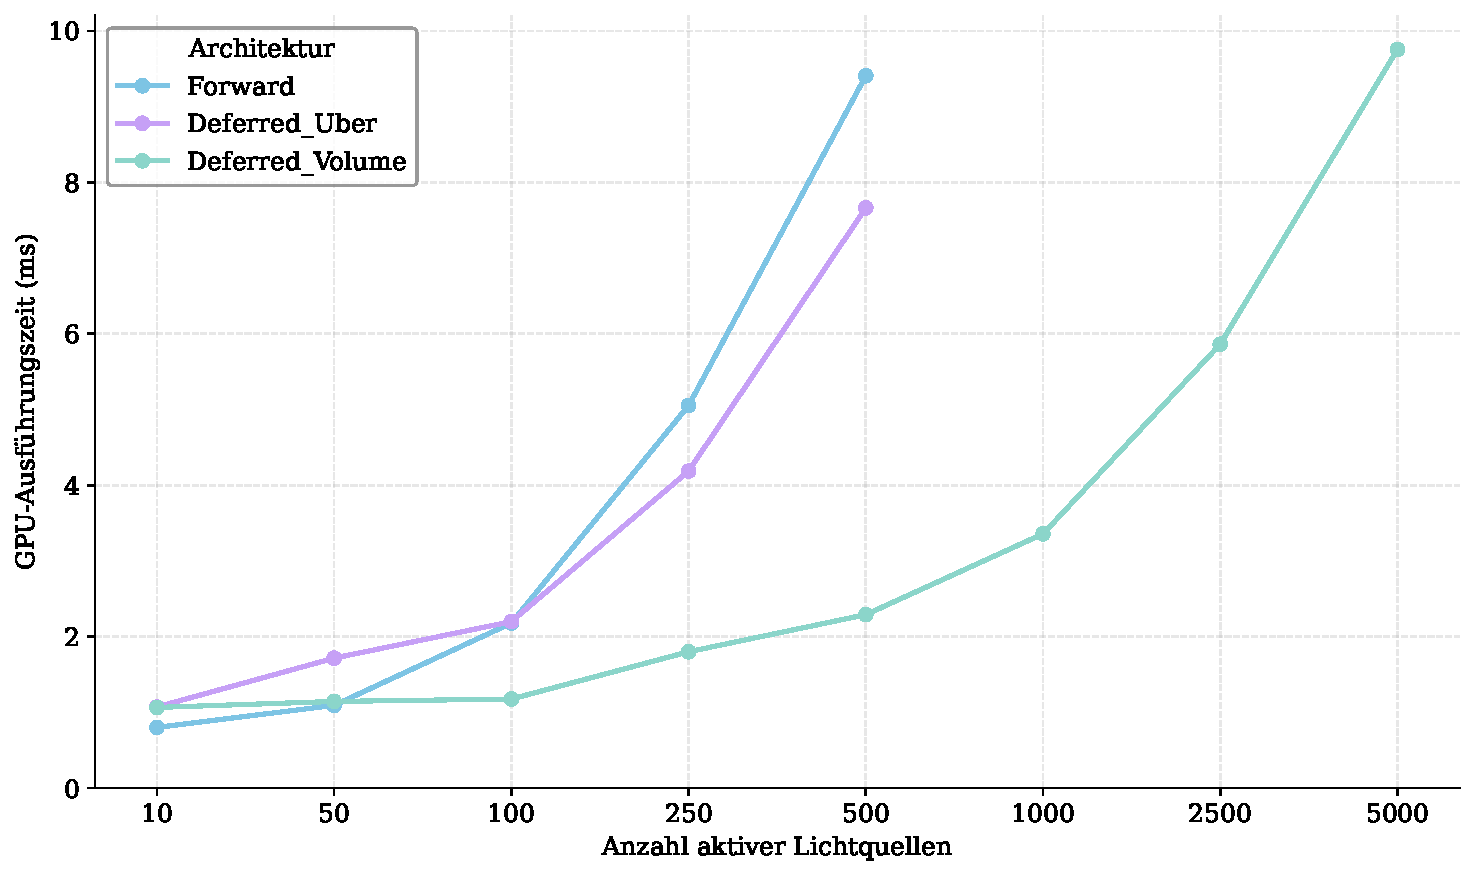
\includegraphics[width=0.9\linewidth]{Abbildungen/5-4-1_LightCount_Means}
    \caption[Skalierung der Lichtanzahl bei dynamischen Punktlichtern]{Messung der GPU-Ausführungszeit in Abhängigkeit
    von der Anzahl aktiver Lichtquellen (10 bis 5.000).}
    \label{fig:5_4_1_light_count_means}
\end{figure}

\subsection{{Lichtintensität \& Overlap}}
\label{subsec:050402_light_intensity_and_overlap_eval}

\begin{figure}[htbp]
    \centering
    
\includegraphics[width=0.9\linewidth]{Abbildungen/5-4-2-1_LightIntensity_Means}
    \caption[Skalierung der Lichtintensität bei konstanter Lichtanzahl]{Messung der GPU-Ausführungszeit in Abhängigkeit
    von der Lichtintensität respektive dem Radius-Multiplikator (0,5 bis 20,0) bei einer konstanten Anzahl von 250
    Lichtquellen.}
    \label{fig:5_4_2_1_light_intensity_means}
\end{figure}

\begin{figure}[htbp]
    \centering
    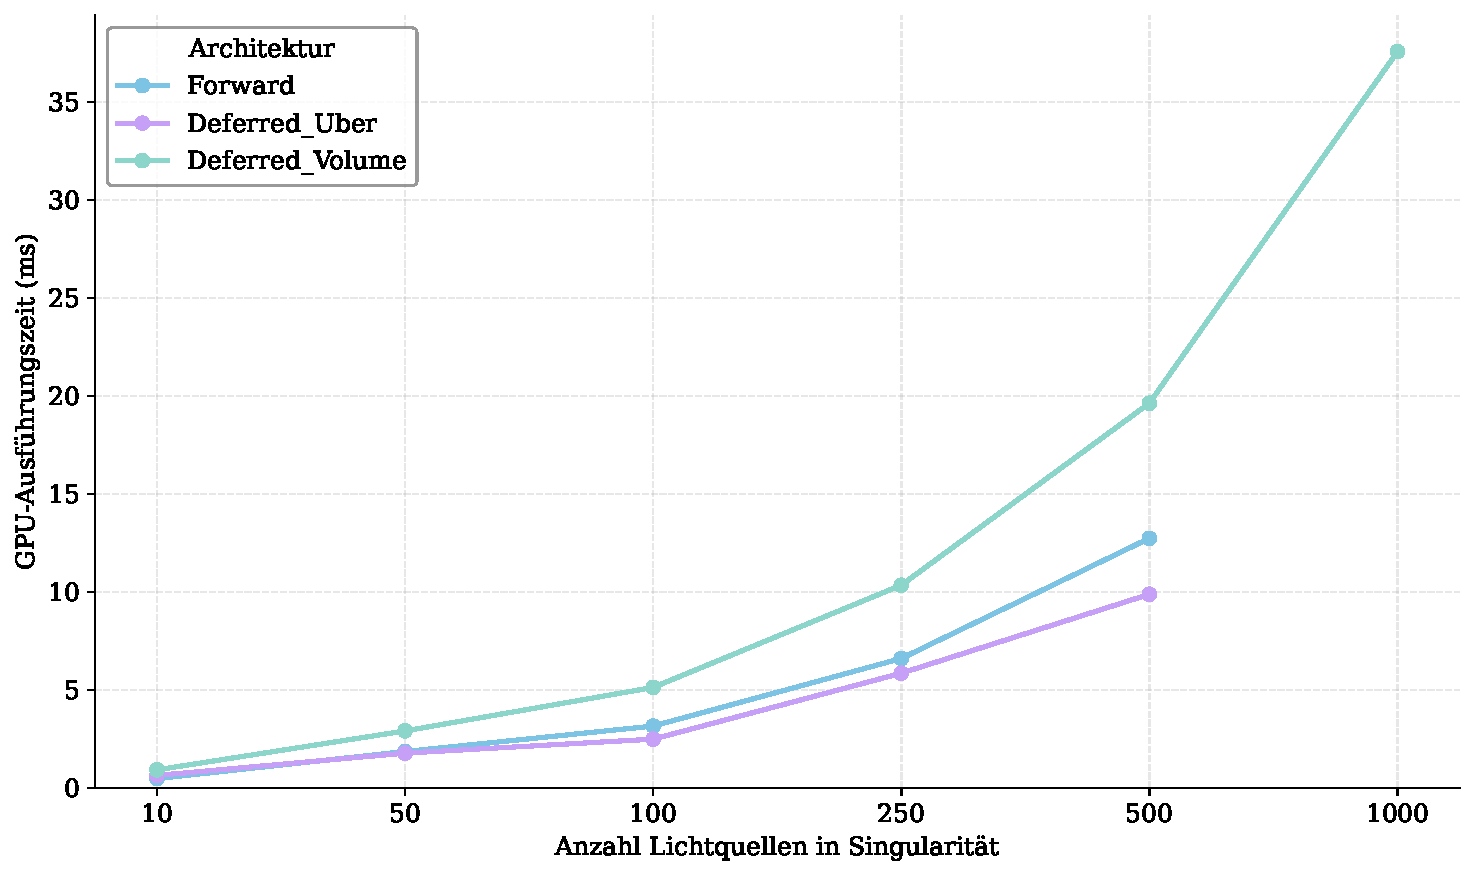
\includegraphics[width=0.9\linewidth]{Abbildungen/5-4-2-2_LightSingularity_Means}
    \caption[Skalierung der Lichtanzahl in einer Singularität]{Messung der GPU-Ausführungszeit in Abhängigkeit von der
    Anzahl der Lichtquellen (10 bis 1000) bei einer Positionierung aller Lichtquellen in einer räumlichen Singularität.}
    \label{fig:5_4_2_2_light_singularity_means}
\end{figure}

\subsection{{Shading Overdraw}}
\label{subsec:050403_shading_overdraw_eval}

\begin{figure}[htbp]
    \centering
    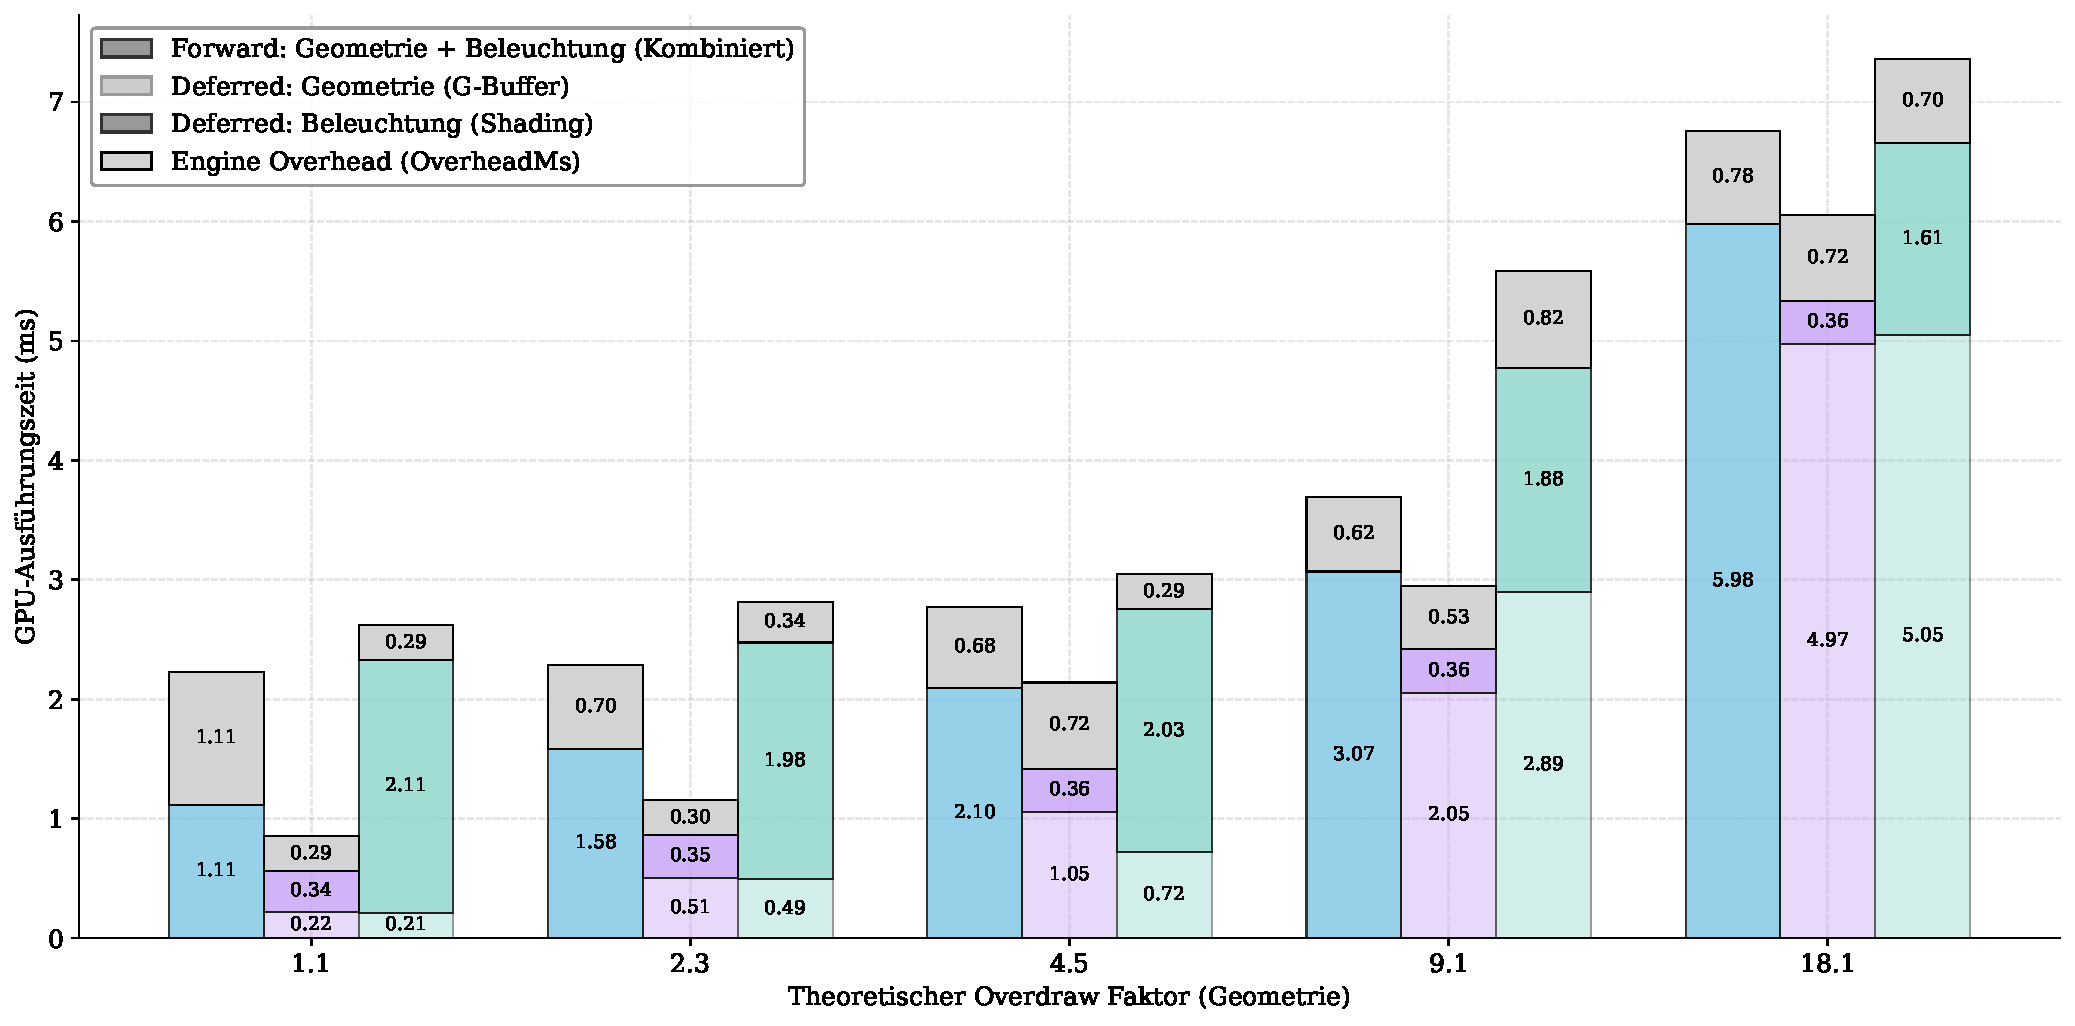
\includegraphics[width=0.9\linewidth]{Abbildungen/5_4_3_decoupling_proof}
    \caption[Entkopplungsnachweis bei steigendem geometrischen Overdraw]{Aufschlüsselung der GPU-Ausführungszeit nach
    einzelnen Pipeline-Komponenten in Abhängigkeit vom theoretischen Overdraw-Faktor bei einer konstanten Last von 100
    Lichtquellen.}
    \label{fig:5_4_3_decoupling_proof}
\end{figure}


\section{{Hybride Stilisierung \& Entropie}}
\label{sec:0505_npr_eval}

In den vorangegangenen Kapiteln 5.2 bis 5.4 wurde das grundlegende Verhalten der evaluierten Rendering-Architekturen
aufgezeigt und somit zugleich die Fähigkeiten und Grenzen des HyDra-Frameworks als Kontrollgruppen demonstriert.
Die nachfolgenden Tests widmen sich dem Kern der Forschung und evaluieren die Wechselwirkungen von Stil-Entropie und
den allgemeinen Einfluss selektiver NPR-Techniken auf die verschiedenen Pipelines.
Der Fokus liegt hierbei insbesondere auf der Evaluation von Warp Divergence und Register Pressure.

\subsection{{Stil-Entropie}}
\label{subsec:050501_entropy_eval}

\begin{figure}[htbp]
    \centering
    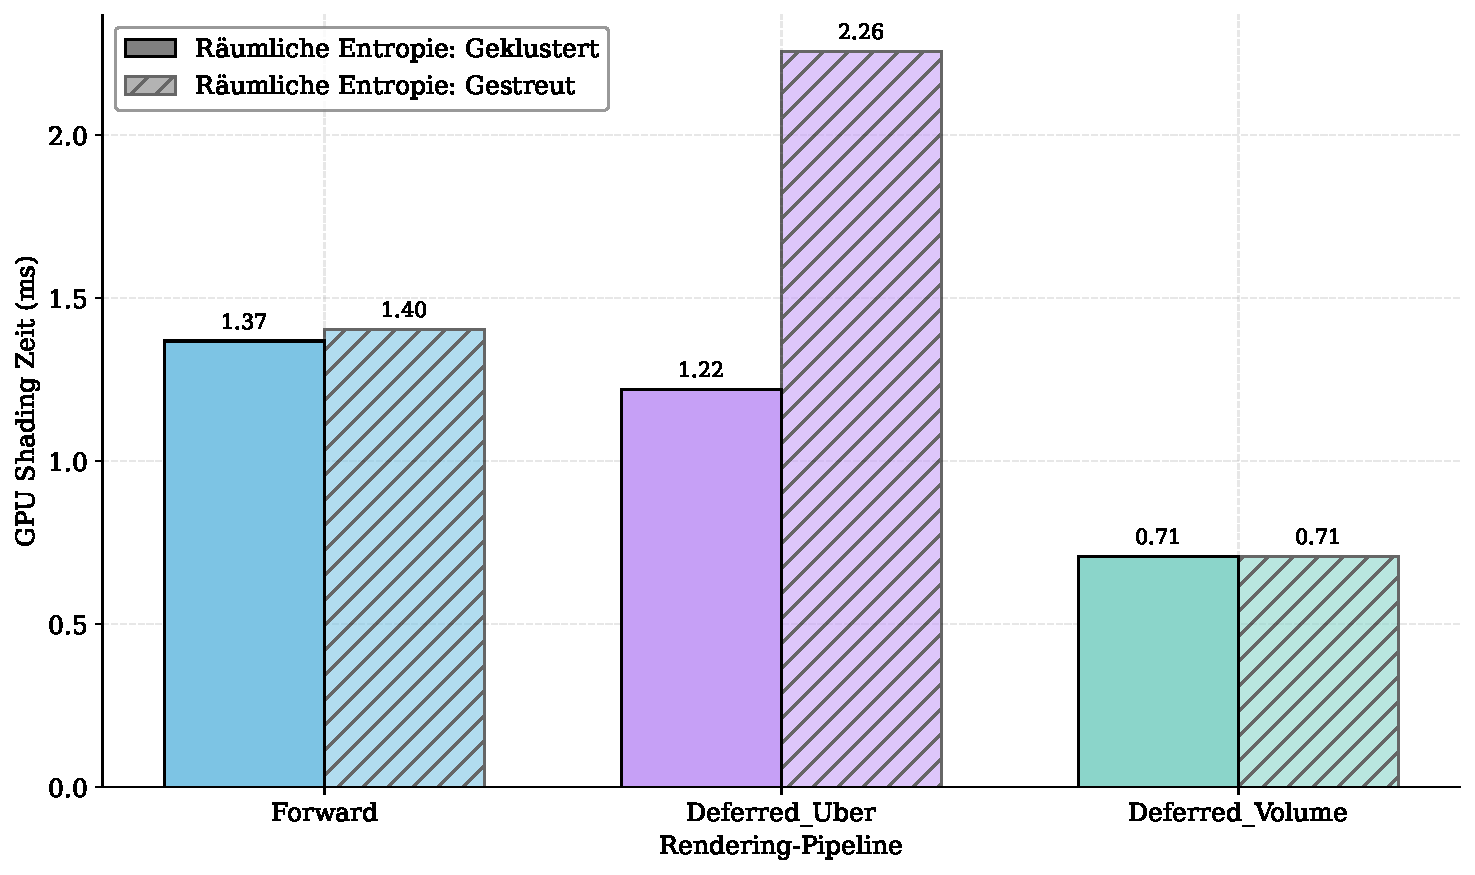
\includegraphics[width=0.9\linewidth]{Abbildungen/5_5_1_entropy_divergence_means}
    \caption[Einfluss der räumlichen Entropie auf die GPU-Shading-Zeit]{Messung der GPU-Shading-Zeit in Abhängigkeit von
    der räumlichen Verteilung (Geklustert vs. Gestreut) der Rendering-Stile zur Isolation von Warp Divergence.}
    \label{fig:5_5_1_entropy_divergence_means}
\end{figure}

\begin{figure}[htbp]
    \centering
    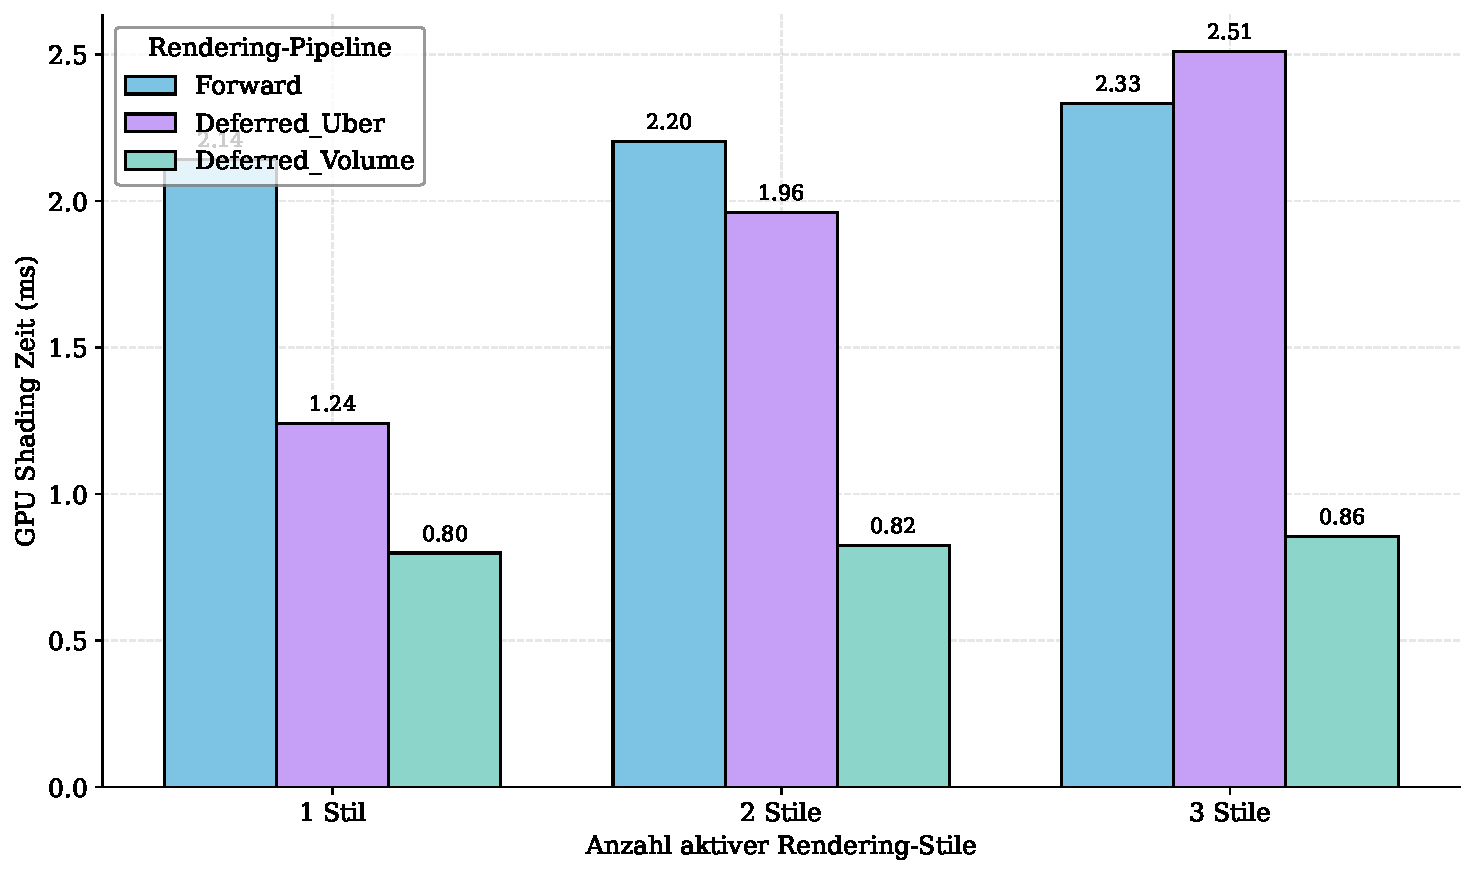
\includegraphics[width=0.9\linewidth]{Abbildungen/5_5_2_style_combinatorics_gpu}
    \caption[Einfluss stilistischer Kombinatorik auf die GPU-Shading-Zeit]{Messung der GPU-Shading-Zeit in Abhängigkeit
    von der Anzahl simultan aktiver Rendering-Stile (1 bis 3 Stile) zur Evaluierung kombinatorischer Degradation.}
    \label{fig:5_5_2_style_combinatorics_gpu}
\end{figure}

\subsection{{Kernel Bandbreiten Limits}}
\label{subsec:050502_kernel_eval}

\begin{figure}[htbp]
    \centering
    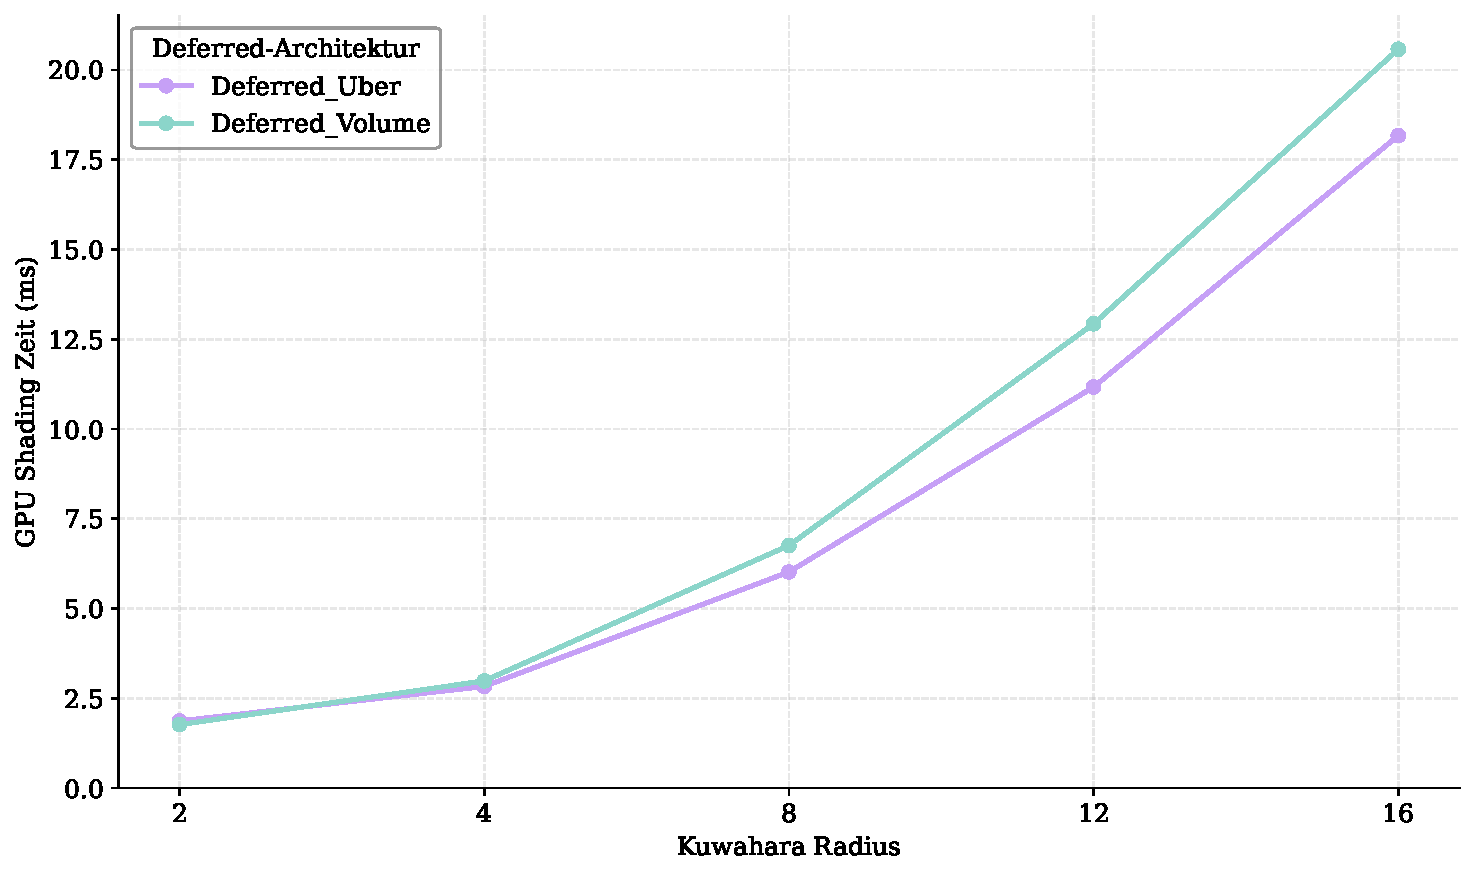
\includegraphics[width=0.9\linewidth]{Abbildungen/5_5_3_kernel_bandwidth_scalability}
    \caption[Skalierung des Kuwahara-Filterradius]{Messung der GPU-Shading-Zeit in Abhängigkeit vom
    Kuwahara-Kernel-Radius (2 bis 16) zur Evaluation der VRAM-Bandbreitenlimits unter steigender Filtergröße.}
    \label{fig:5_5_3_kernel_bandwidth_scalability}
\end{figure}


\section{{Macro-Benchmark Synthese}}
\label{sec:0506_kernel_eval}

In der finalen Testreihe erfolgt die Integration aller übergeordneter Einflüsse aus den vorangegangenen Benchmarks in
ein umfassendes Real-World-Szenario, um die Interaktion der bislang untersuchten Effekte in ihrer Gesamtheit zu
analysieren.
Die nachfolgenden Evaluationen werden in einem Schritt zusammengefasst, bestehen allerdings aus vier verschiedenen
Einzelpässen, in welchen die verschiedenen Einflüsse von Geometrie, Beleuchtung und selektiver Silisierung gemeinsam
betrachtet werden.

\begin{figure}[htbp]
    \centering
    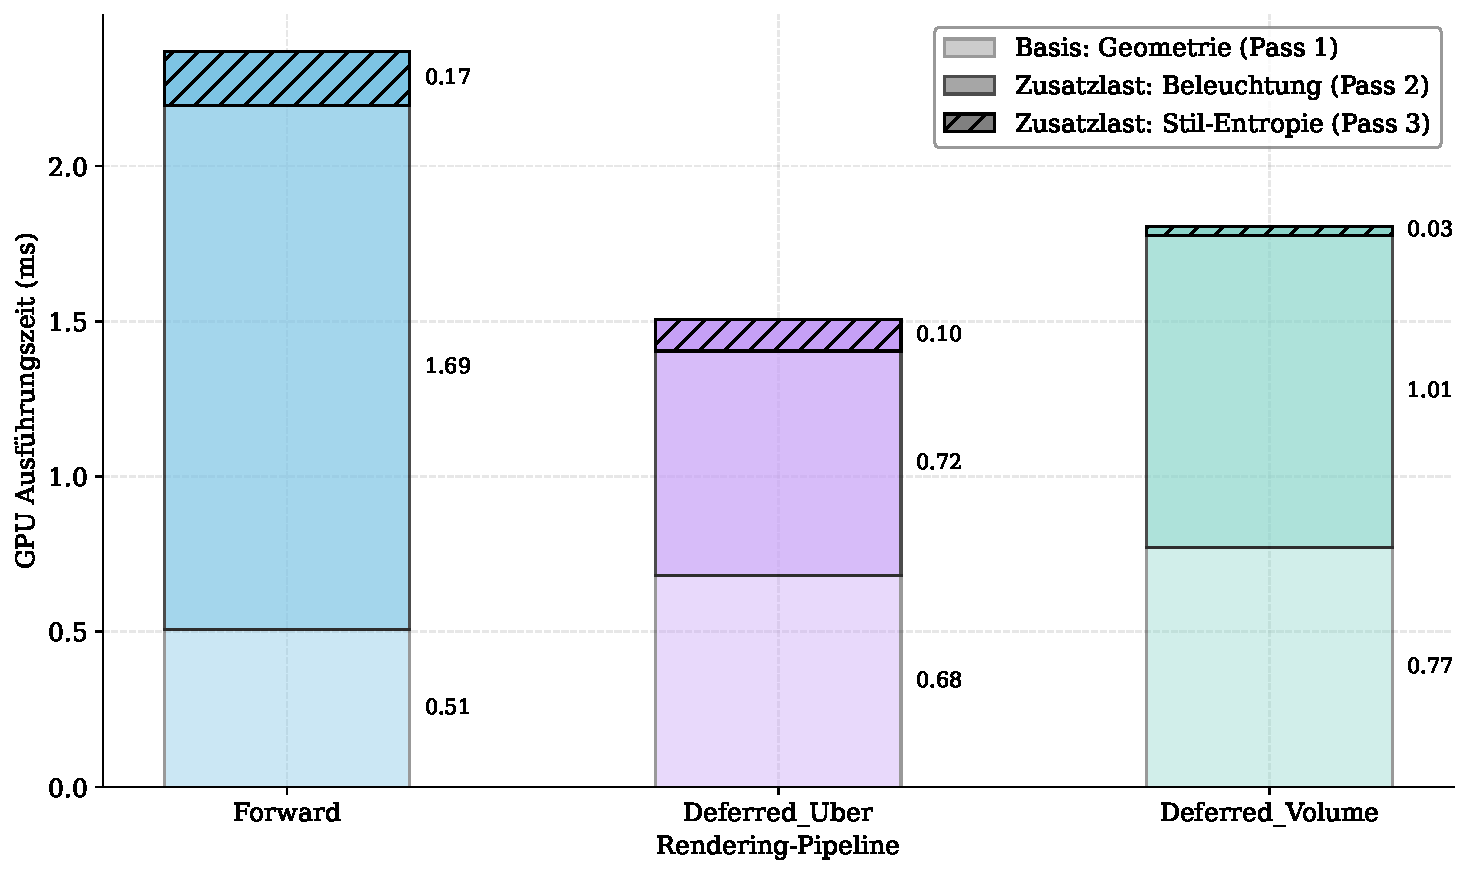
\includegraphics[width=0.9\linewidth]{Abbildungen/5_6_cumulative_rendering_cost_combined}
    \caption[Akkumulierte GPU-Ausführungszeit im Makro-Benchmark]{Aufschlüsselung der GPU-Ausführungszeit nach
    Pipeline-Komponenten (Geometrie, Beleuchtung und Stil-Entropie).}
    \label{fig:5_6_cumulative_rendering_cost_combined}
\end{figure}

\begin{figure}[htbp]
    \centering
    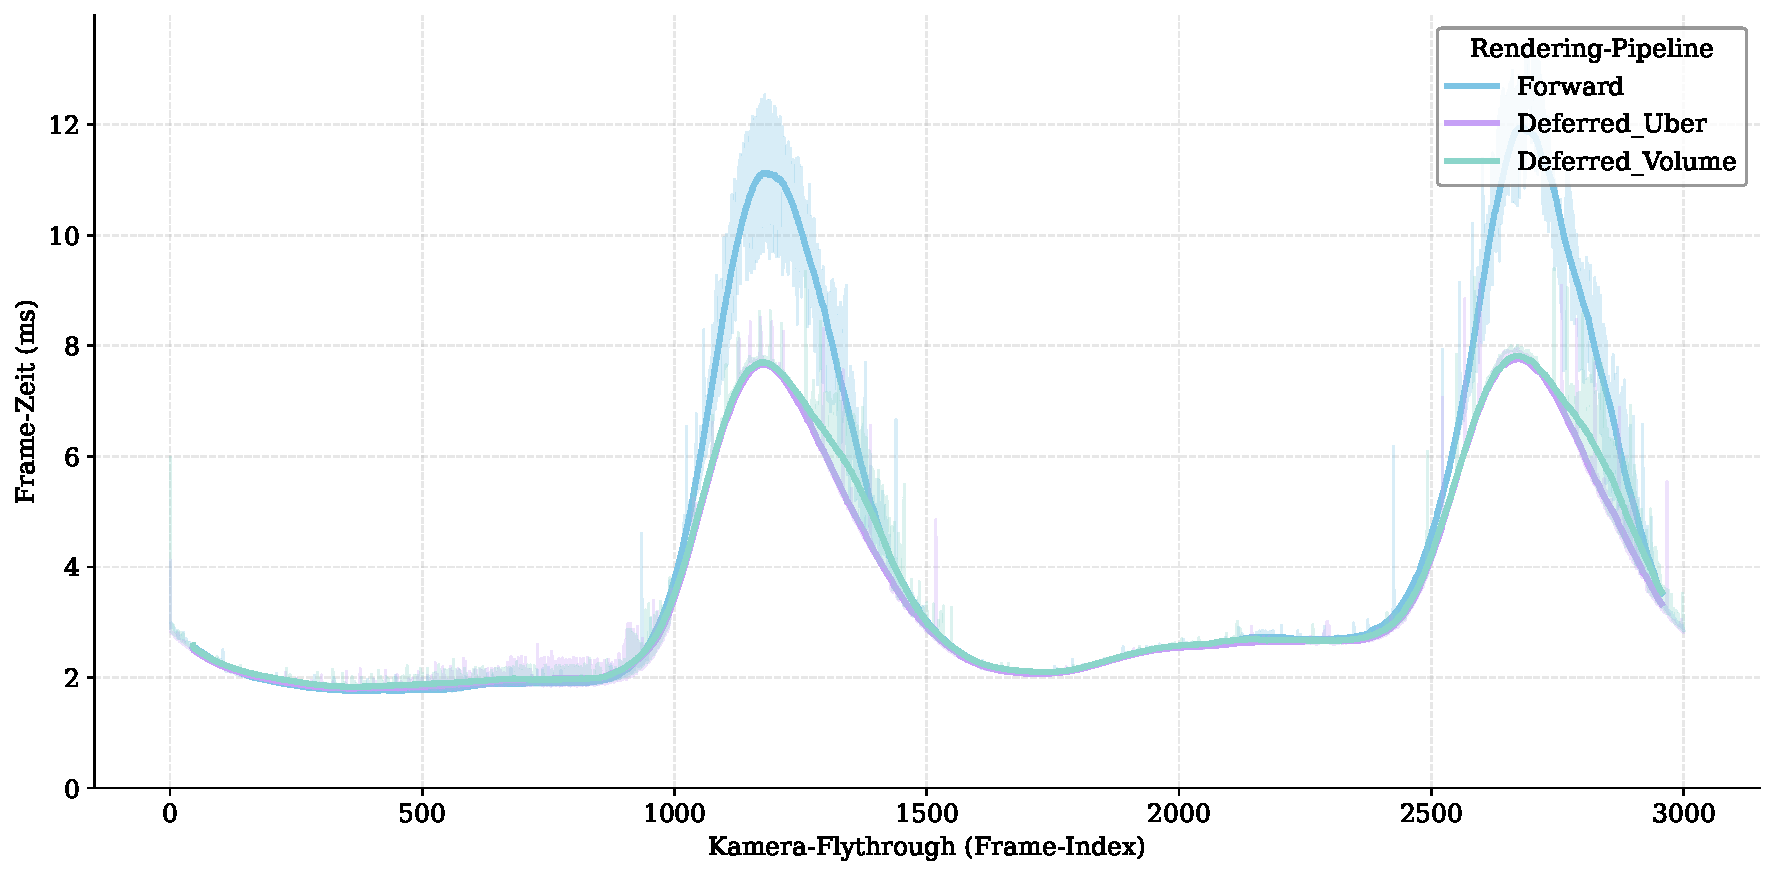
\includegraphics[width=0.9\linewidth]{Abbildungen/5_6_flythrough_variance}
    \caption[Frame-Zeit-Verlauf des Kamera-Flythroughs]{Verlauf der Frame-Zeit über die Dauer von 3000 Frames des
    Kamera-Flythroughs unter kombinierter Geometrie-, Beleuchtungs- und Stil-Last.}
    \label{fig:5_6_flythrough_variance}
\end{figure}


    % 8-12 Seiten
    \chapter{Diskussion}
\label{ch:06_diskussion}

Dieses Kapitel führt die theoretischen Anforderungen und die praktischen Messergebnisse zusammen. Der Fokus liegt auf der Bewertung der Daten, der Vorstellung der heuristischen Entscheidungsmatrix als Kernbeitrag der Arbeit sowie einer kritischen Betrachtung der eigenen Arbeitsweise und der Erfahrungen bei der Entwicklung.


\section{Zusammenführung und Interpretation der Testergebnisse}
\label{sec:0601_interpretation_results}

Abgleich der gemessenen Kurven mit den zuvor aufgestellten Vermutungen aus den Tests. Beschreibung der genauen Belastungsgrenzen aller drei Render-Wege bei steigender Last durch Lichter, Geometriedichte und durcheinandergewürfelte Zeichenstile im Bild.


\section{Die heuristische Entscheidungsmatrix}
\label{sec:0602_heuristic_matrix}

Vorstellung des eigentlichen Ergebnisses der Arbeit in Form einer übersichtlichen Entscheidungsmatrix für Entwickler. Bereitstellung von konkreten Empfehlungen für den Aufbau einer Grafik-Engine basierend auf Geometriedichte, Lichtanzahl und gewünschten Zeichenstilen, wobei die Matrix in der praktischen Anwendung wie ein Kochbuch Schritt für Schritt durch die Architekturentscheidung führt.


\section{Kritische Reflexion und Limitationen}
\label{sec:0603_limitations}

Ehrliche Betrachtung der Schwachstellen und Grenzen des gewählten Versuchsaufbaus. Diskussion über bewusst weggelassene Faktoren wie andere Lichttypen, transparente Objekte oder die Ausführung auf mobilen Geräten und deren Auswirkung auf die Aussagekraft der Messergebnisse.


\section{Lessons Learned}
\label{sec:0604_lessons_learned_engineering}

Betrachtung von Nutzen und Aufwand aus Sicht der Softwareentwicklung abseits der reinen Performance-Messwerte. Vergleich zwischen der schwierigen Wartung von sehr großen Shader-Dateien und der besseren Modularität anderer Ansätze sowie Probleme beim fehlerfreien Einbau der Zeitmessung.

    % 2-3 Seiten
    \chapter{Zusammenfassung und Ausblick}
\label{ch:07_zusammenfassung_ausblick}

Dieses abschließende Kapitel fasst die gesamte Arbeit kurz zusammen und gibt einen Ausblick auf zukünftige Entwicklungen.


\section{Resümee der Arbeit}
\label{sec:0701_resuemee}

Kurzer Rückblick auf die ursprüngliche Herausforderung und das Ziel der Arbeit. Zusammenfassung der Entwicklung des Test-Frameworks und der wichtigsten Erkenntnisse über das Zusammenspiel von Geometriedichte, Lichtanzahl und der Vielfalt von Zeichenstilen. Abschließende Beschreibung des Nutzens der erstellten heuristischen Entscheidungsmatrix für die Praxis.


\section{Ausblick und zukünftige Arbeiten}
\label{sec:0702_future_work}

Konkrete Vorschläge für die technologische Weiterentwicklung des Programms. Ideen für den Einbau neuerer Render-Verfahren, um die gefundenen Hardware-Grenzen aufzuheben. Vorschläge für zusätzliche Test-Szenarien mit komplexeren Lichttypen, prozeduralen Materialien sowie für die Untersuchung von Bildfehlern und modernen Methoden der Kantenglättung.

    \clearpage

    % --- Zone 4: Kleine römische Zahlen (i, ii, iii...) ---
    \setcounter{page}{1}
    \pagenumbering{roman}

    % Literatur & Anhang
    \printbibliography
    \clearpage

    \appendix
    % \input{Kapitel/09_Anhang}

\end{document}